\subsection{Giao diện bắt đầu}
\begin{figure}[H]
    \centering
    % Hình 1 bên trái
    \begin{subfigure}[b]{0.45\textwidth} % Độ rộng chiếm 45% chiều rộng văn bản
        \centering
        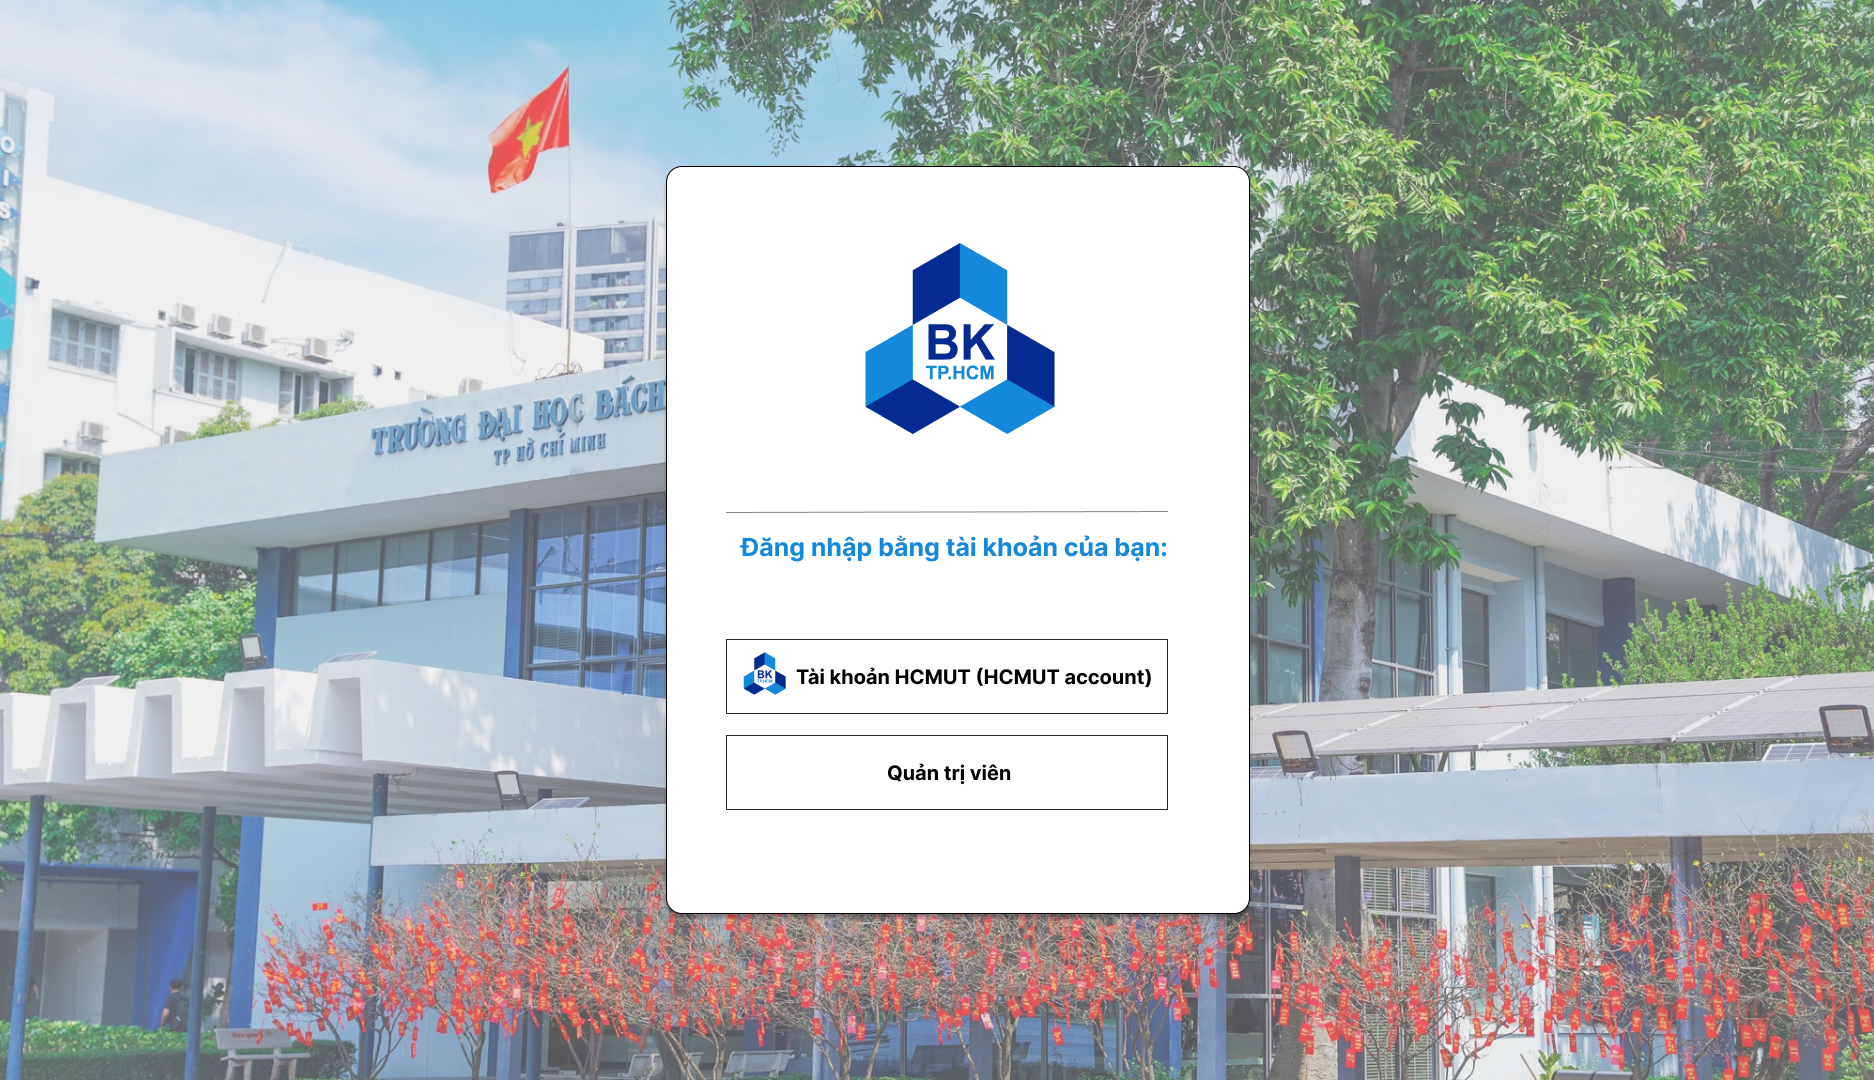
\includegraphics[width=\linewidth]{pictures/Login1.png}
        \caption{Giao diện đăng nhập đầu tiên}
        \label{fig:statechart1}
    \end{subfigure}
    \hfill % Khoảng trống linh hoạt giữa hai hình
    % Hình 2 bên phải
    \begin{subfigure}[b]{0.45\textwidth} % Độ rộng chiếm 45% chiều rộng văn bản
        \centering
        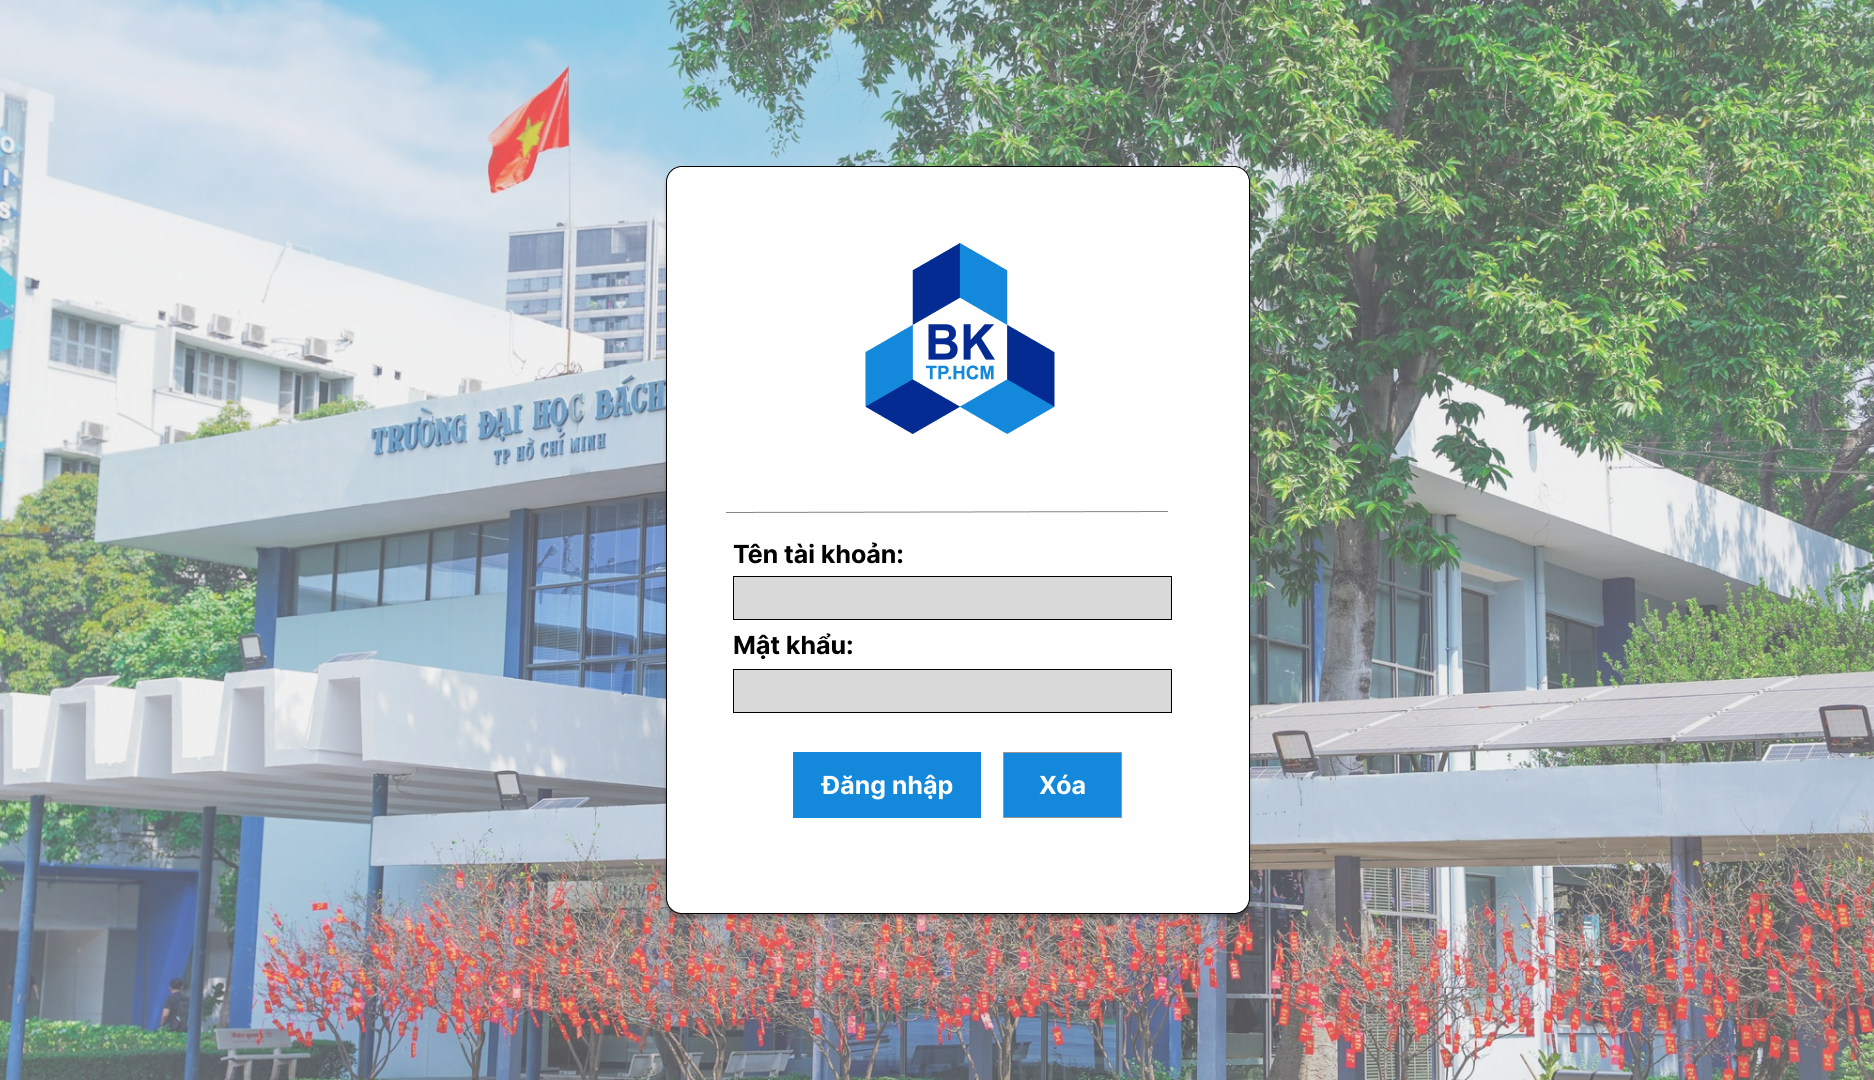
\includegraphics[width=\linewidth]{pictures/Login2.png} % Điều chỉnh width một chút để cân đối hơn nếu cần
        \caption{Giao diện đăng nhập thứ hai}
        \label{fig:statechart2}
    \end{subfigure}
    
    % Chú thích chung cho cả cụm hình (tùy chọn)
    \caption{Ảnh chụp màn hình đăng nhập}
    \label{fig:both_statecharts}
\end{figure}

Giao diện đăng nhập đóng vai trò là điểm chạm đầu tiên và là cửa ngõ tiếp cận toàn bộ hệ thống. Tại đây, mọi người dùng đều phải thực hiện bước xác thực danh tính bằng cách cung cấp các thông tin cơ bản bao gồm tên tài khoản và mật khẩu. Quá trình này đảm bảo tính bảo mật, đồng thời cấp quyền để người dùng có thể truy cập và sử dụng đầy đủ các tính năng mà ứng dụng web cung cấp.

\begin{figure}[H]
    \centering
    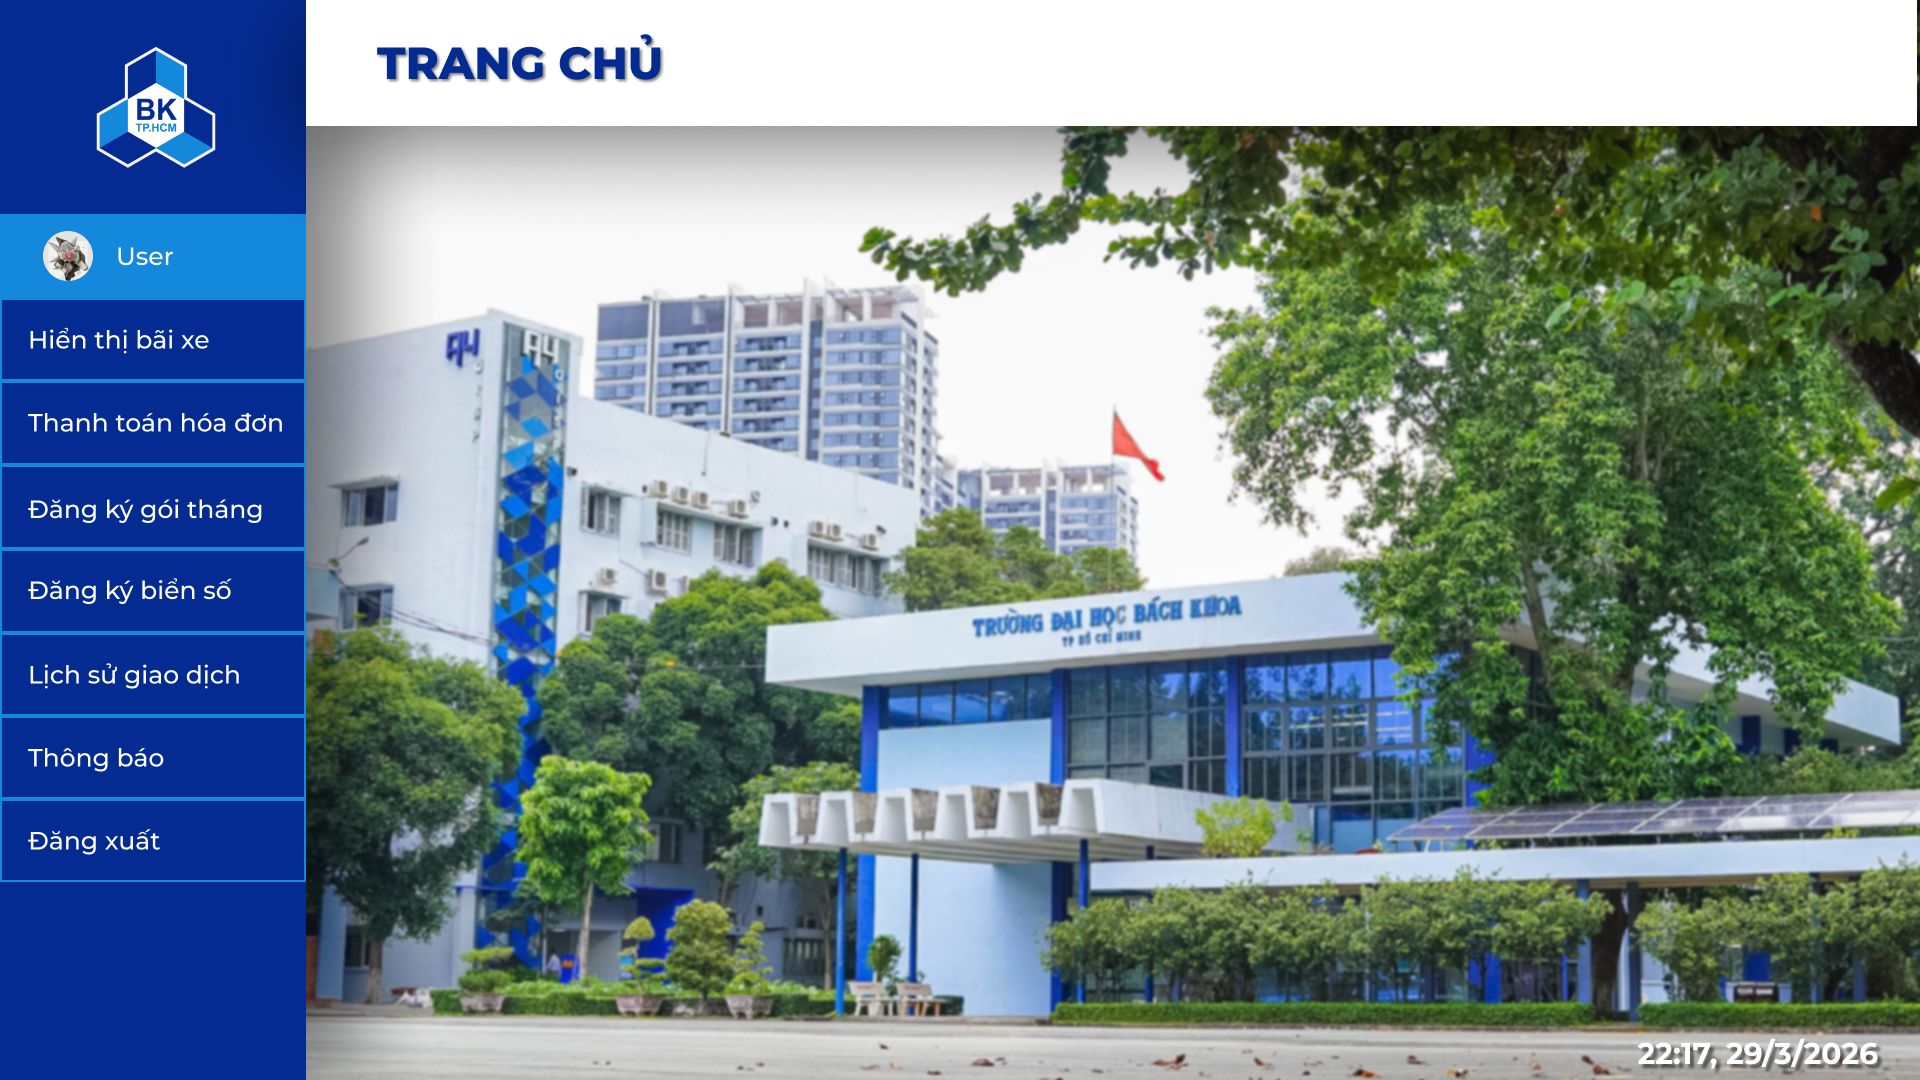
\includegraphics[width=0.6\textwidth]{pictures/Main.png}
    \caption{Giao diện trang chủ web}
\end{figure}

Sau khi hoàn tất quá trình xác thực thành công, hệ thống sẽ tự động điều hướng người dùng đến Trang chủ. Đây được xem là không gian làm việc trung tâm và là điểm kết nối mọi hoạt động trên nền tảng.






\subsection{Giao diện đăng ký biển số xe}

\begin{figure}[H]
    \centering
    % Hàng 1
    \begin{subfigure}[b]{0.45\textwidth}
        \centering
        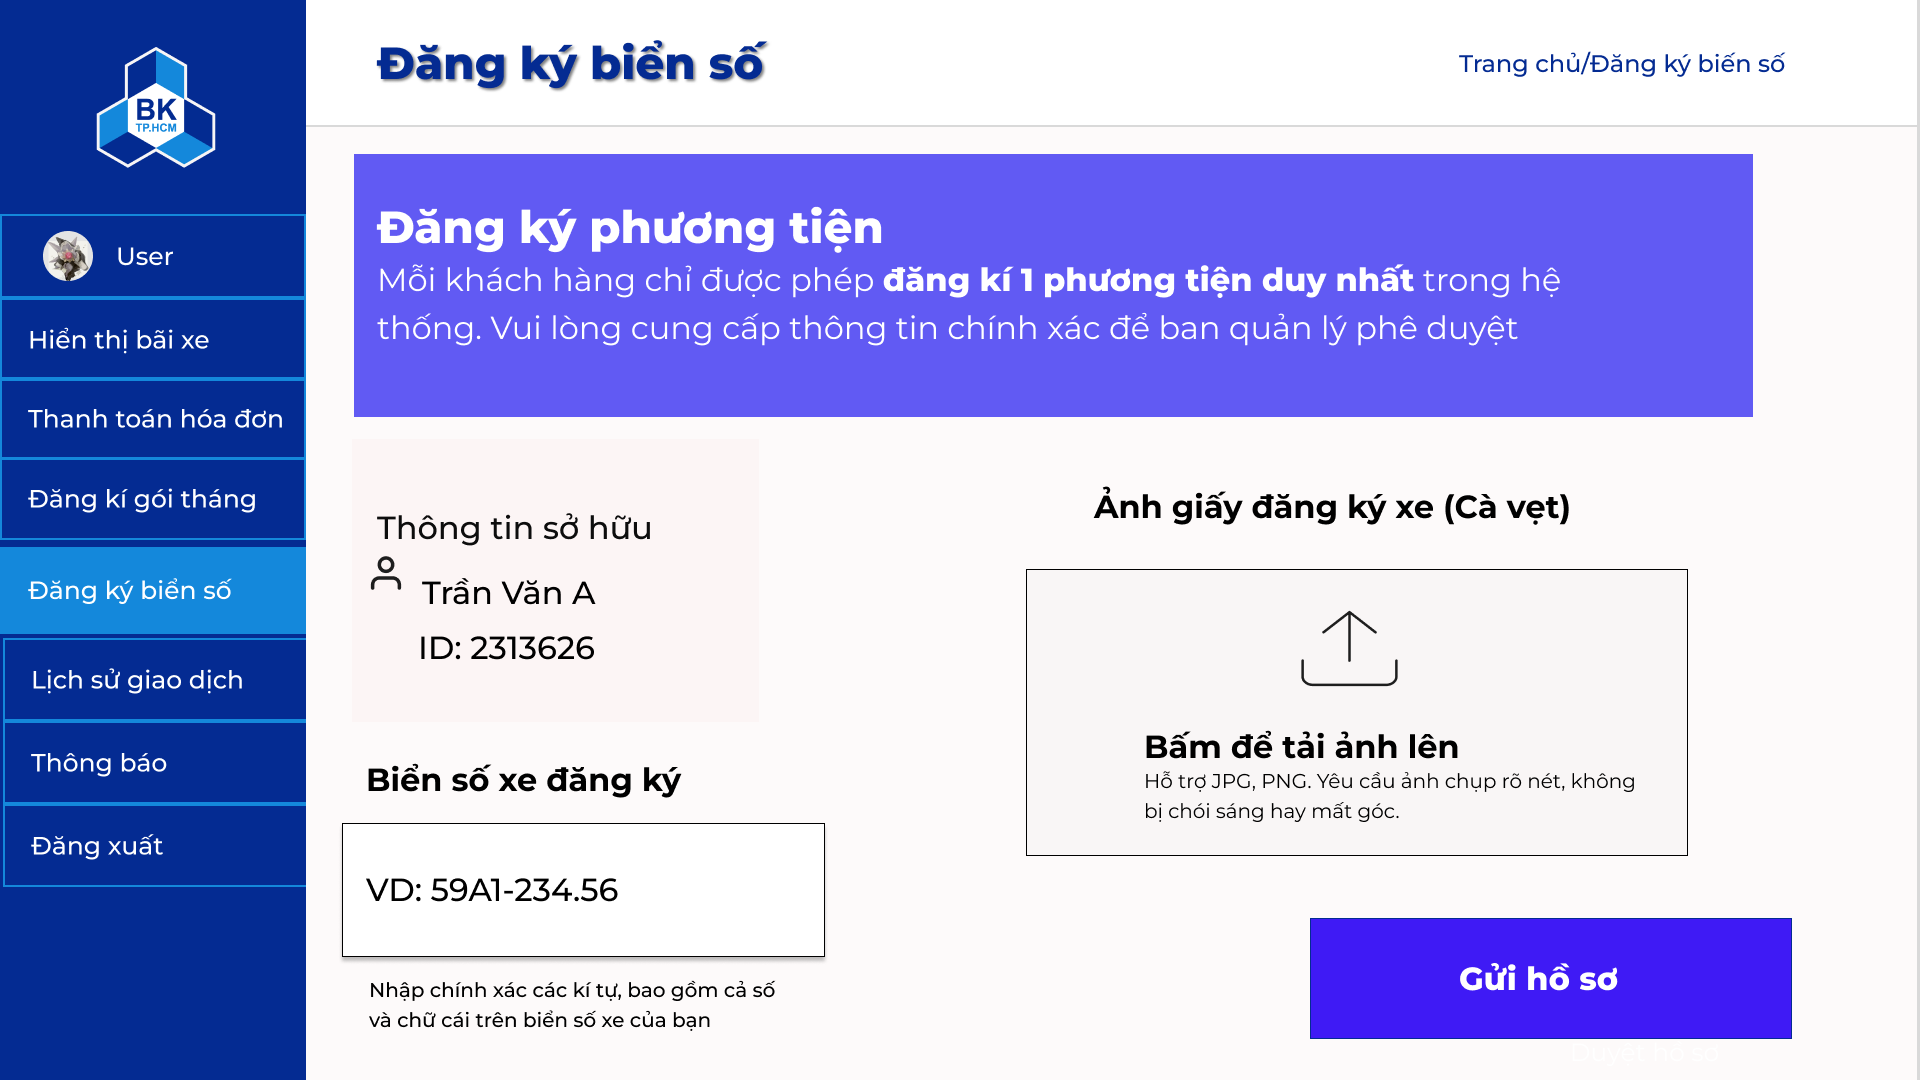
\includegraphics[width=\linewidth]{pictures/DKbienso1.png}
        \caption{Giao diện nhập thông tin đăng ký biến số}
        \label{fig:login1}
    \end{subfigure}
    \hfill
    \begin{subfigure}[b]{0.45\textwidth}
        \centering
        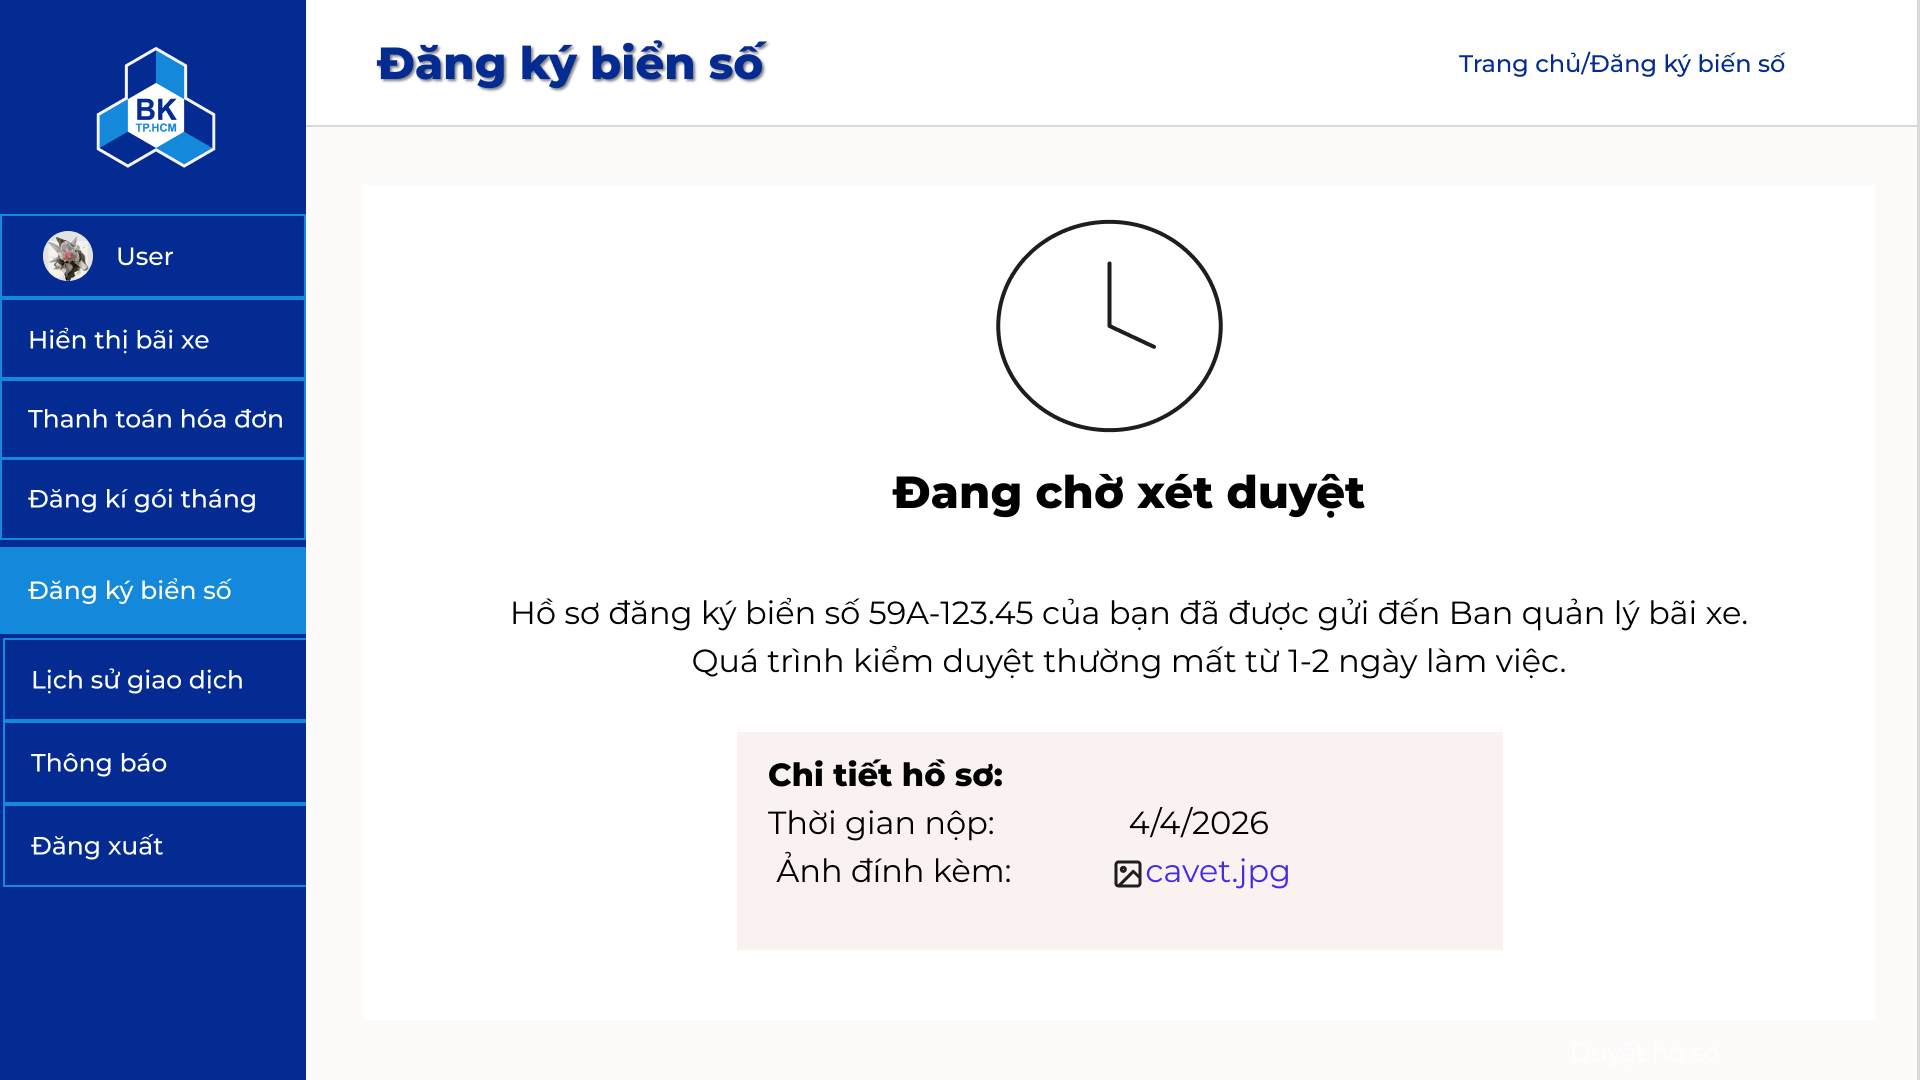
\includegraphics[width=\linewidth]{pictures/DKbienso2.png}
        \caption{Giao diện chờ xét duyệt biển số}
        \label{fig:login2}
    \end{subfigure}

    \vspace{0.5cm} % Tạo khoảng cách nhỏ giữa hàng trên và hàng dưới

    % Hàng 2
    \begin{subfigure}[b]{0.45\textwidth}
        \centering
        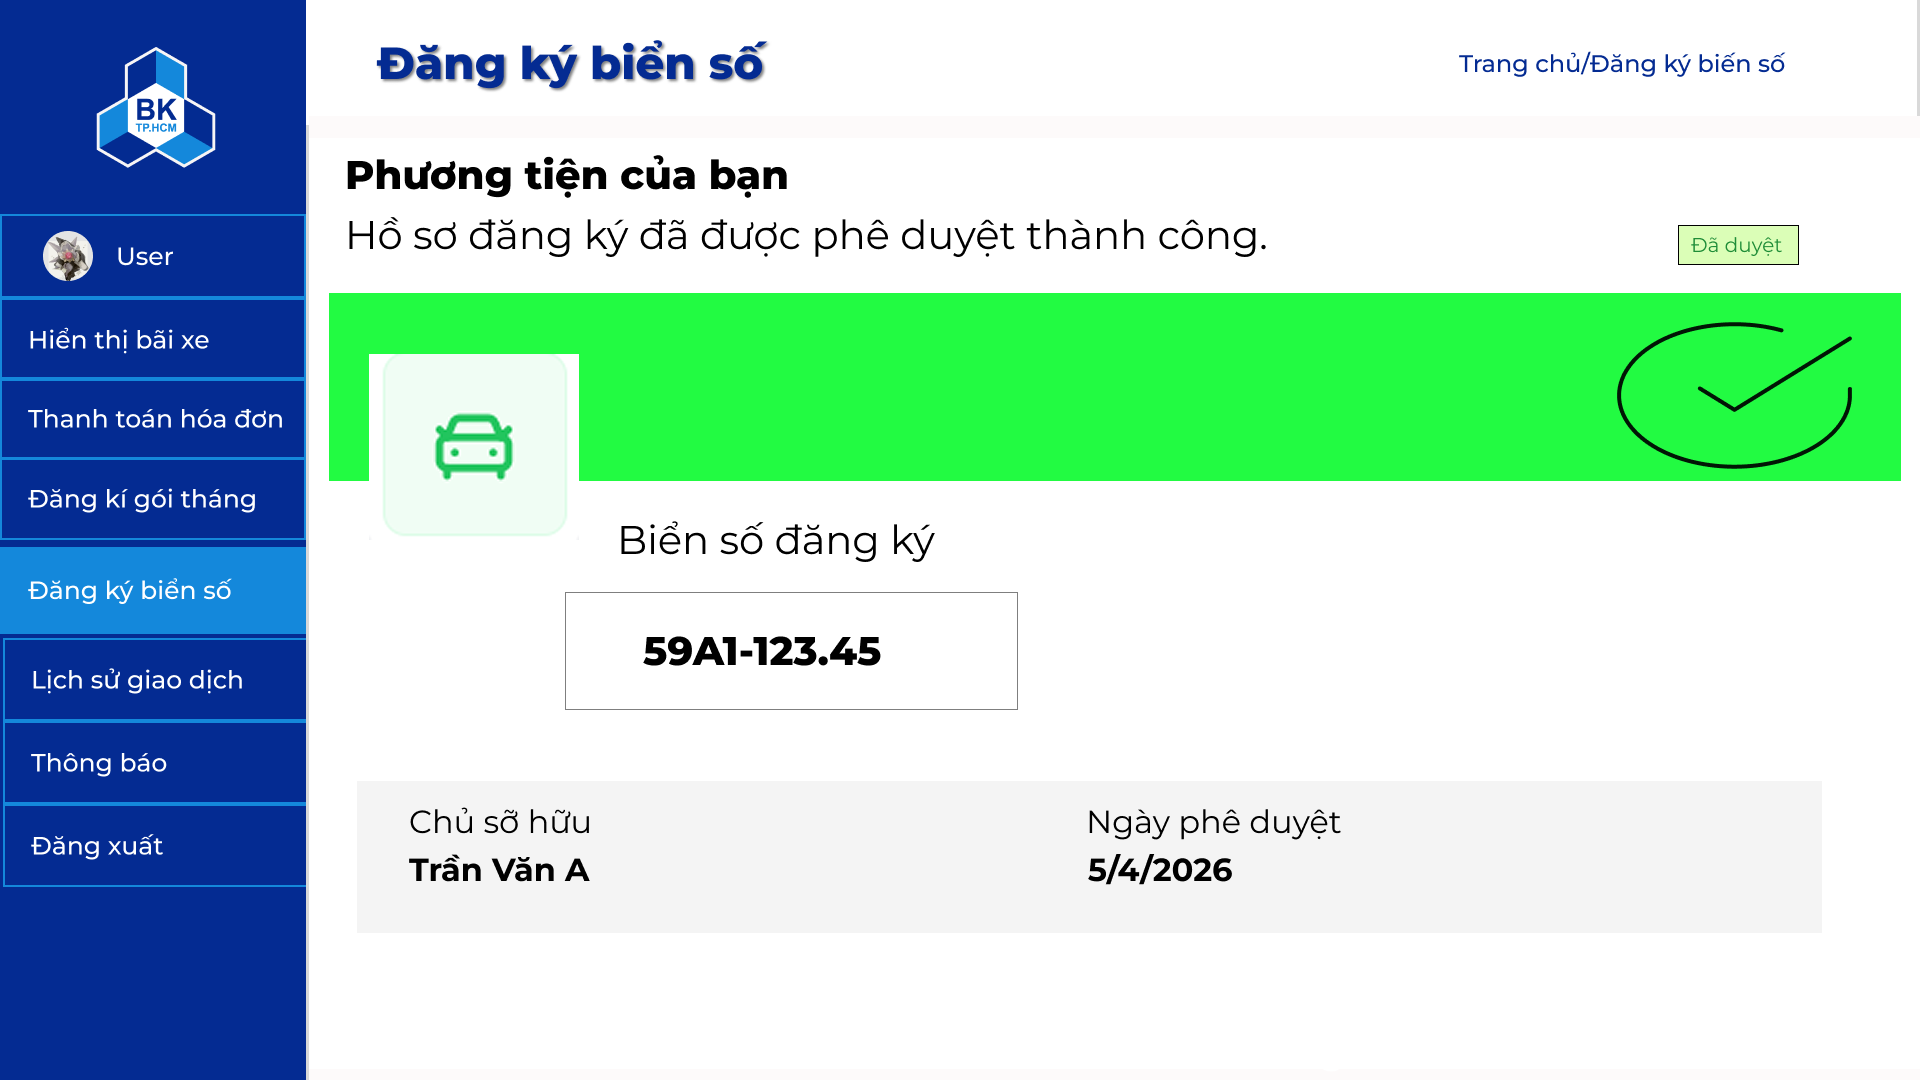
\includegraphics[width=\linewidth]{pictures/DKbienso3.png}
        \caption{Giao diện đăng ký thành công}
        \label{fig:login3}
    \end{subfigure}
    \hfill
    \begin{subfigure}[b]{0.45\textwidth}
        \centering
        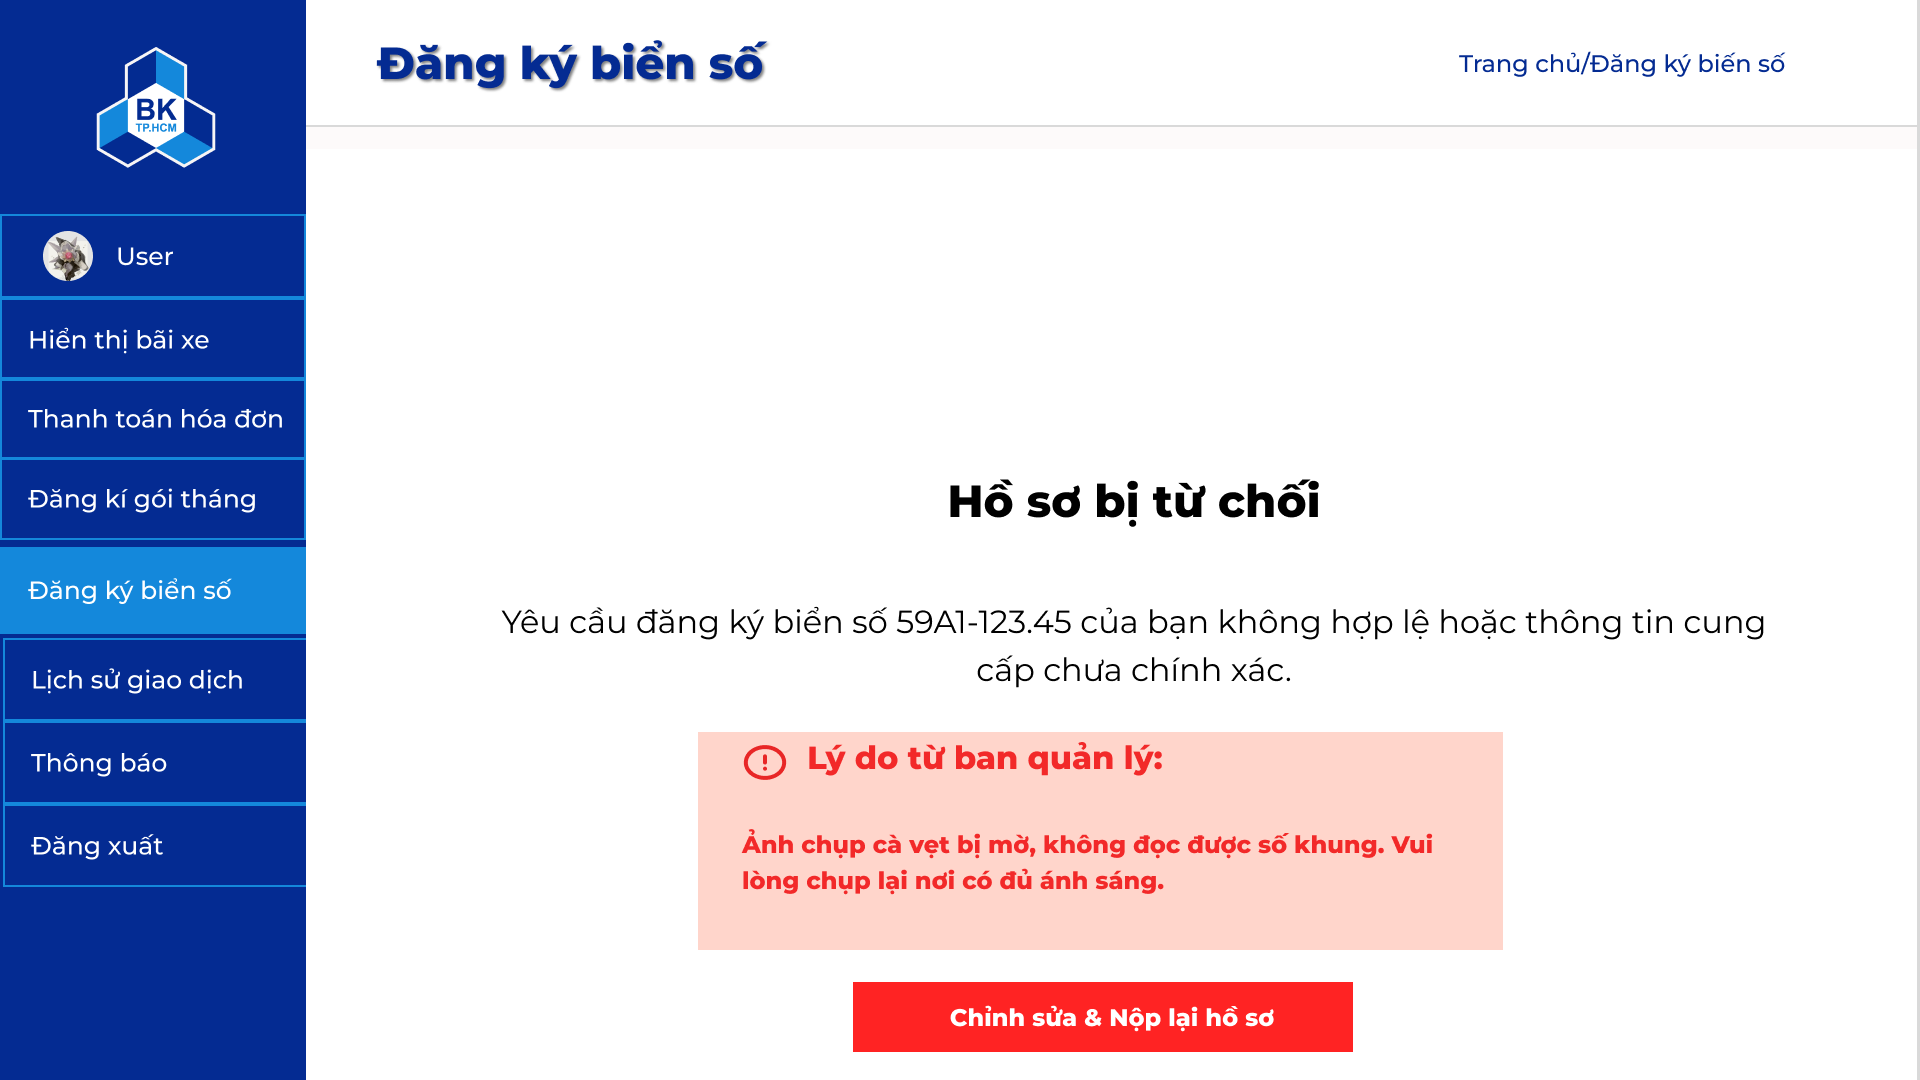
\includegraphics[width=\linewidth]{pictures/DKbienso4.png}
        \caption{Giao diện đăng ký thất bại}
        \label{fig:login4}
    \end{subfigure}
    
    \caption{Tổng hợp giao diện cho các bước đăng ký biển số xe}
    \label{fig:all_logins}
\end{figure}

Để có thể tiếp cận và sử dụng trọn vẹn các dịch vụ tiện ích mà hệ thống cung cấp, điều quan trọng nhất là người dùng phải thực hiện đăng ký phương tiện cá nhân. Phần trên đây sẽ trình bày chi tiết các màn hình sẽ xuất hiện trong quy trình khai báo và đăng ký biển số xe vào cơ sở dữ liệu của trang web.

\begin{figure}[H]
    \centering
    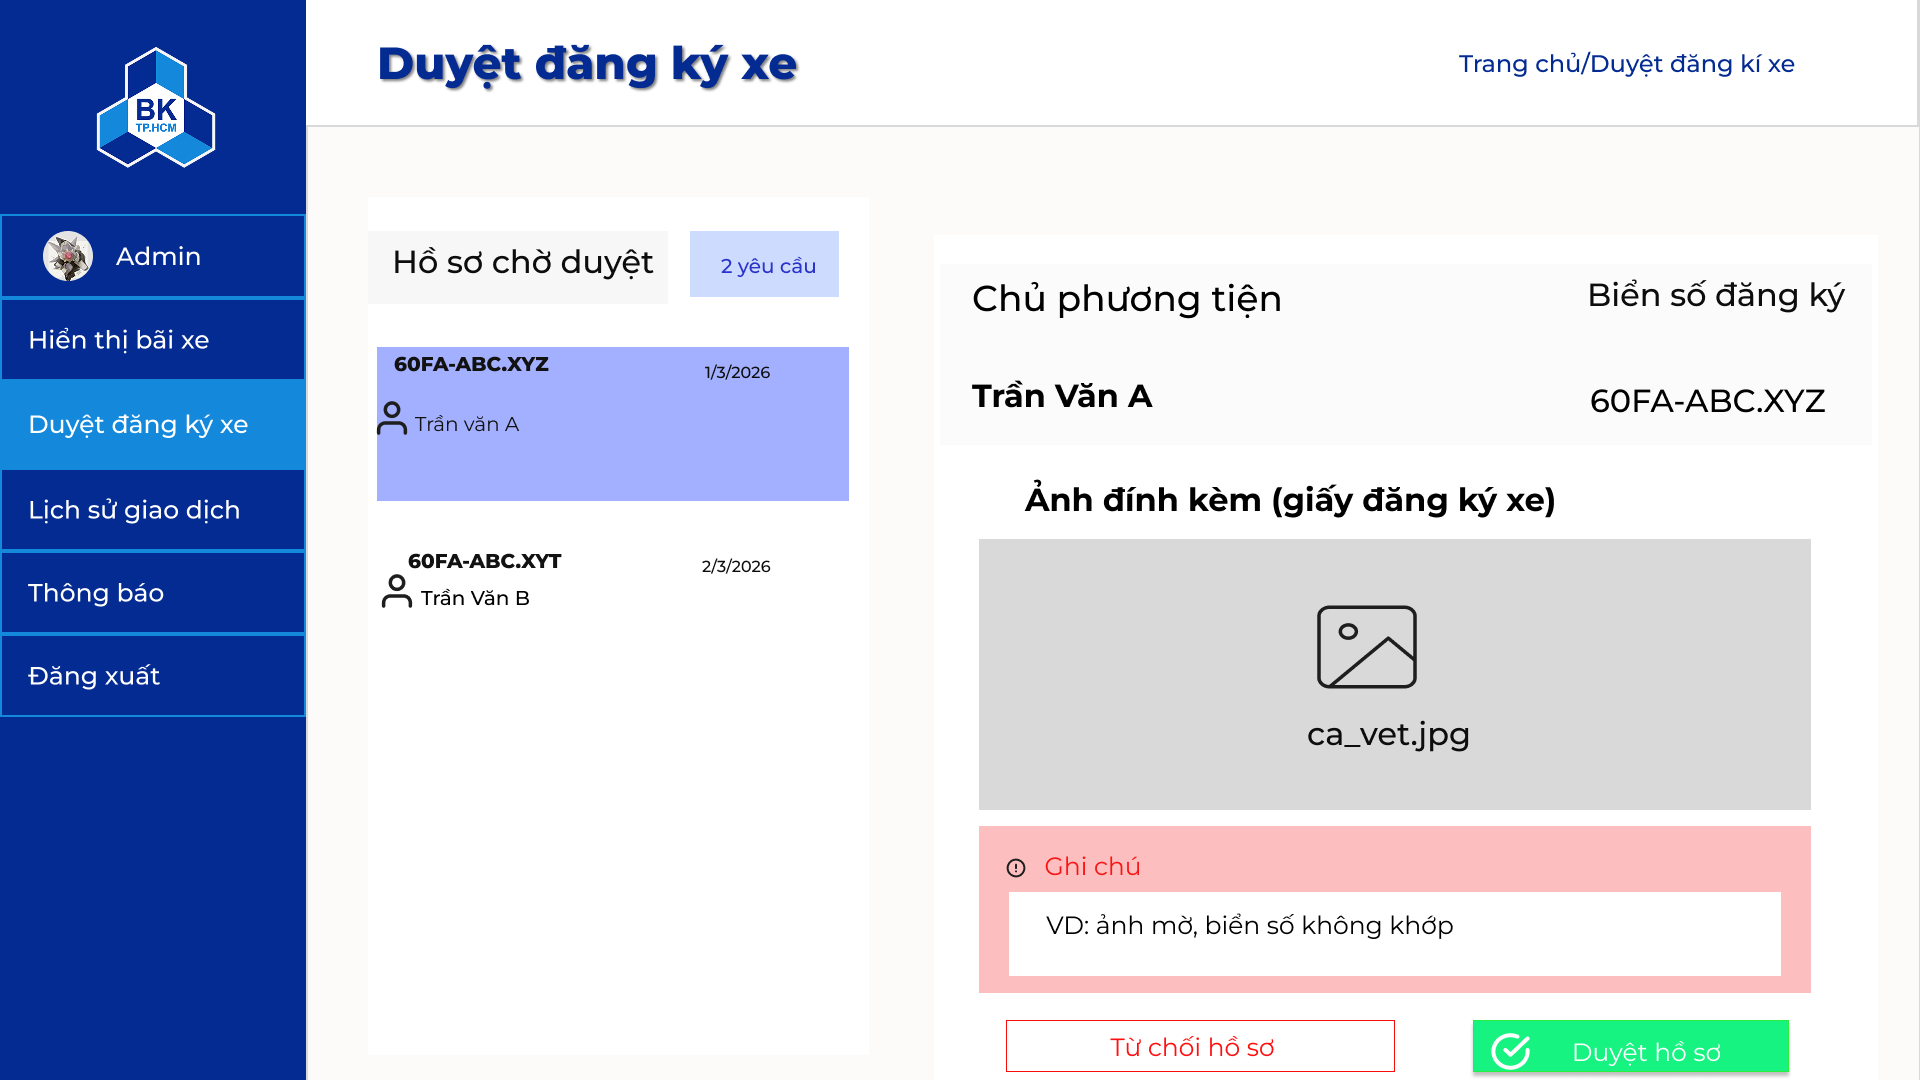
\includegraphics[width=0.6\textwidth]{pictures/DKbienso5.png}
    \caption{Giao diện xét duyệt đăng ký biển số bên phía nhân viên}
\end{figure}

Ngay sau khi người dùng hoàn tất thủ tục gửi yêu cầu đăng ký, dữ liệu sẽ được hệ thống tiếp nhận và chuyển giao sang phân hệ quản trị. Tại đây, đội ngũ nhân viên sẽ được cung cấp một giao diện màn hình chuyên biệt để tiến hành quy trình kiểm tra, xác minh và xét duyệt tính hợp lệ của hồ sơ phương tiện.




\subsection{Các giao diện cho các tiện ích khác của người dùng}

\begin{figure}[H]
    \centering
    
    % Hàng 1: 2 ảnh
    \begin{subfigure}[b]{0.45\textwidth}
        \centering
        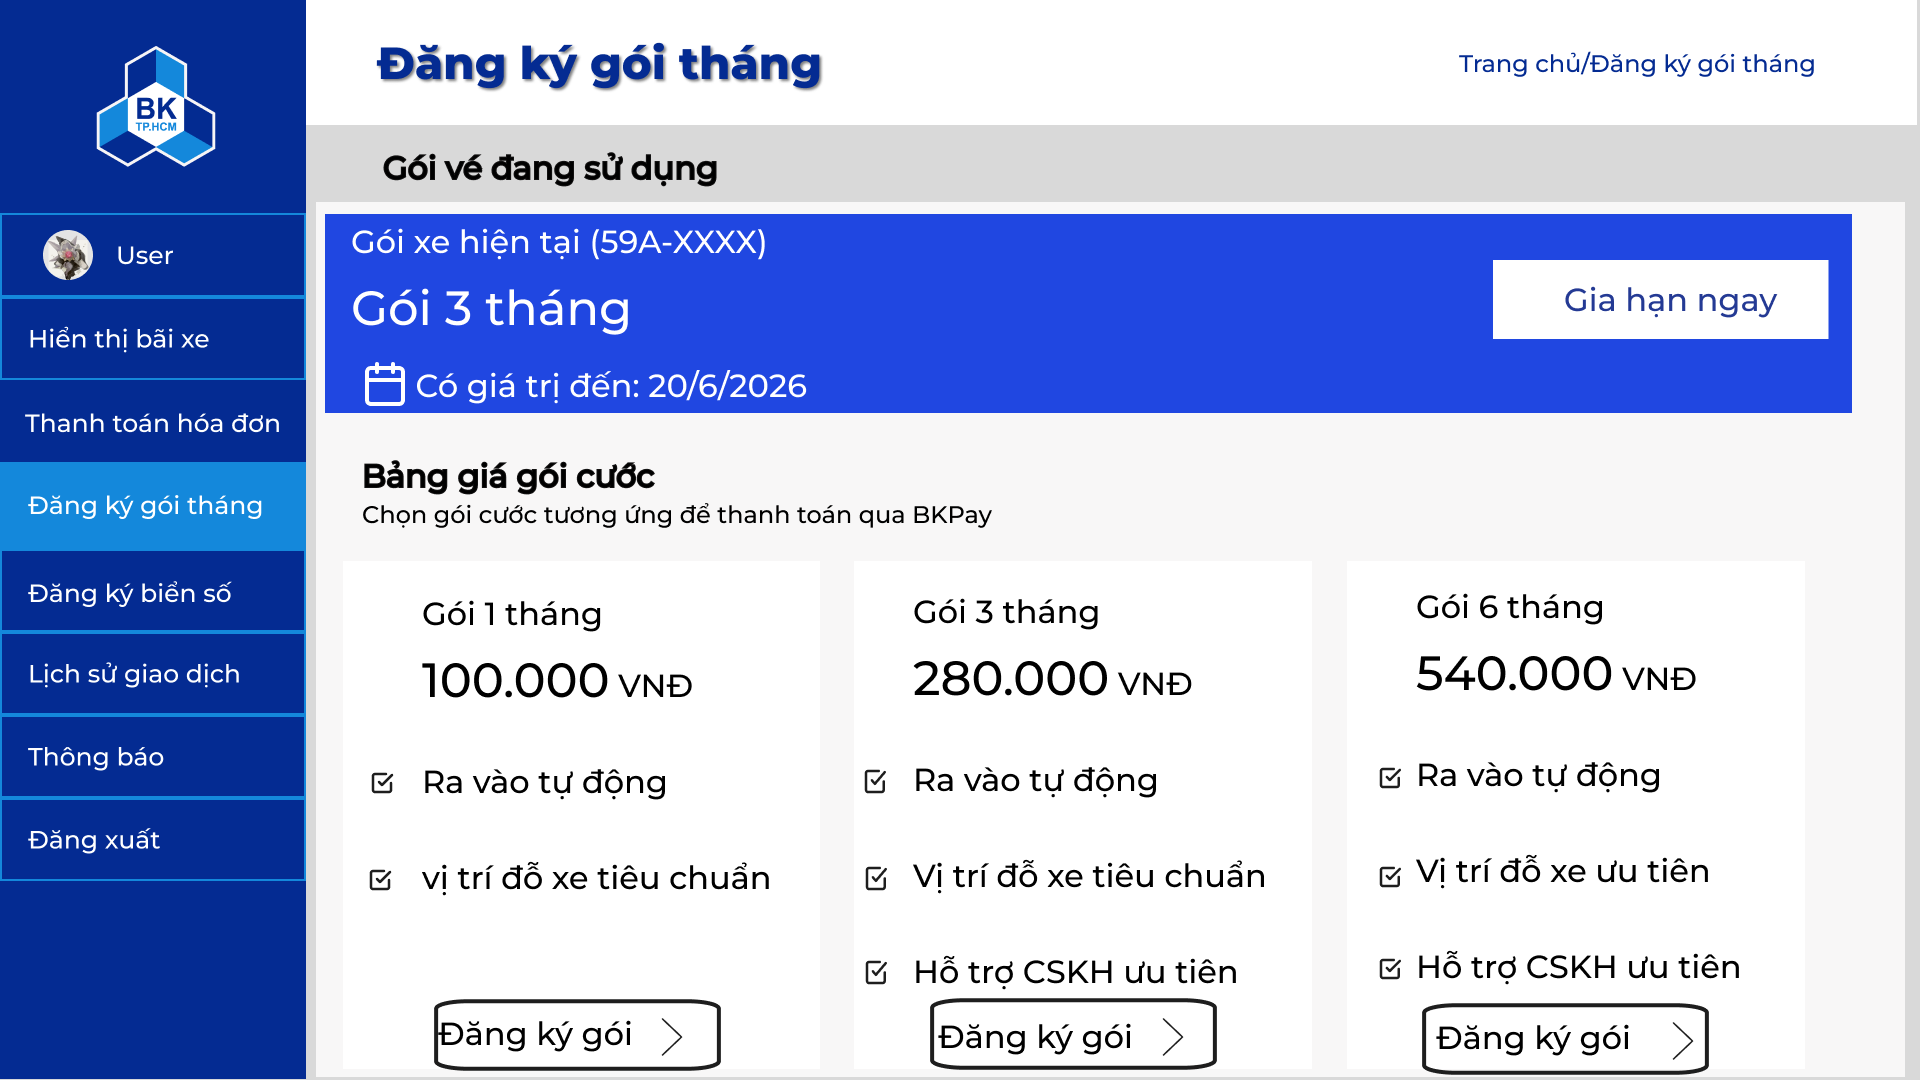
\includegraphics[width=\linewidth]{pictures/DKthang.png}
        \caption{Giao diện đăng ký gói tháng}
        \label{fig:login1}
    \end{subfigure}
    \hfill
    \begin{subfigure}[b]{0.45\textwidth}
        \centering
        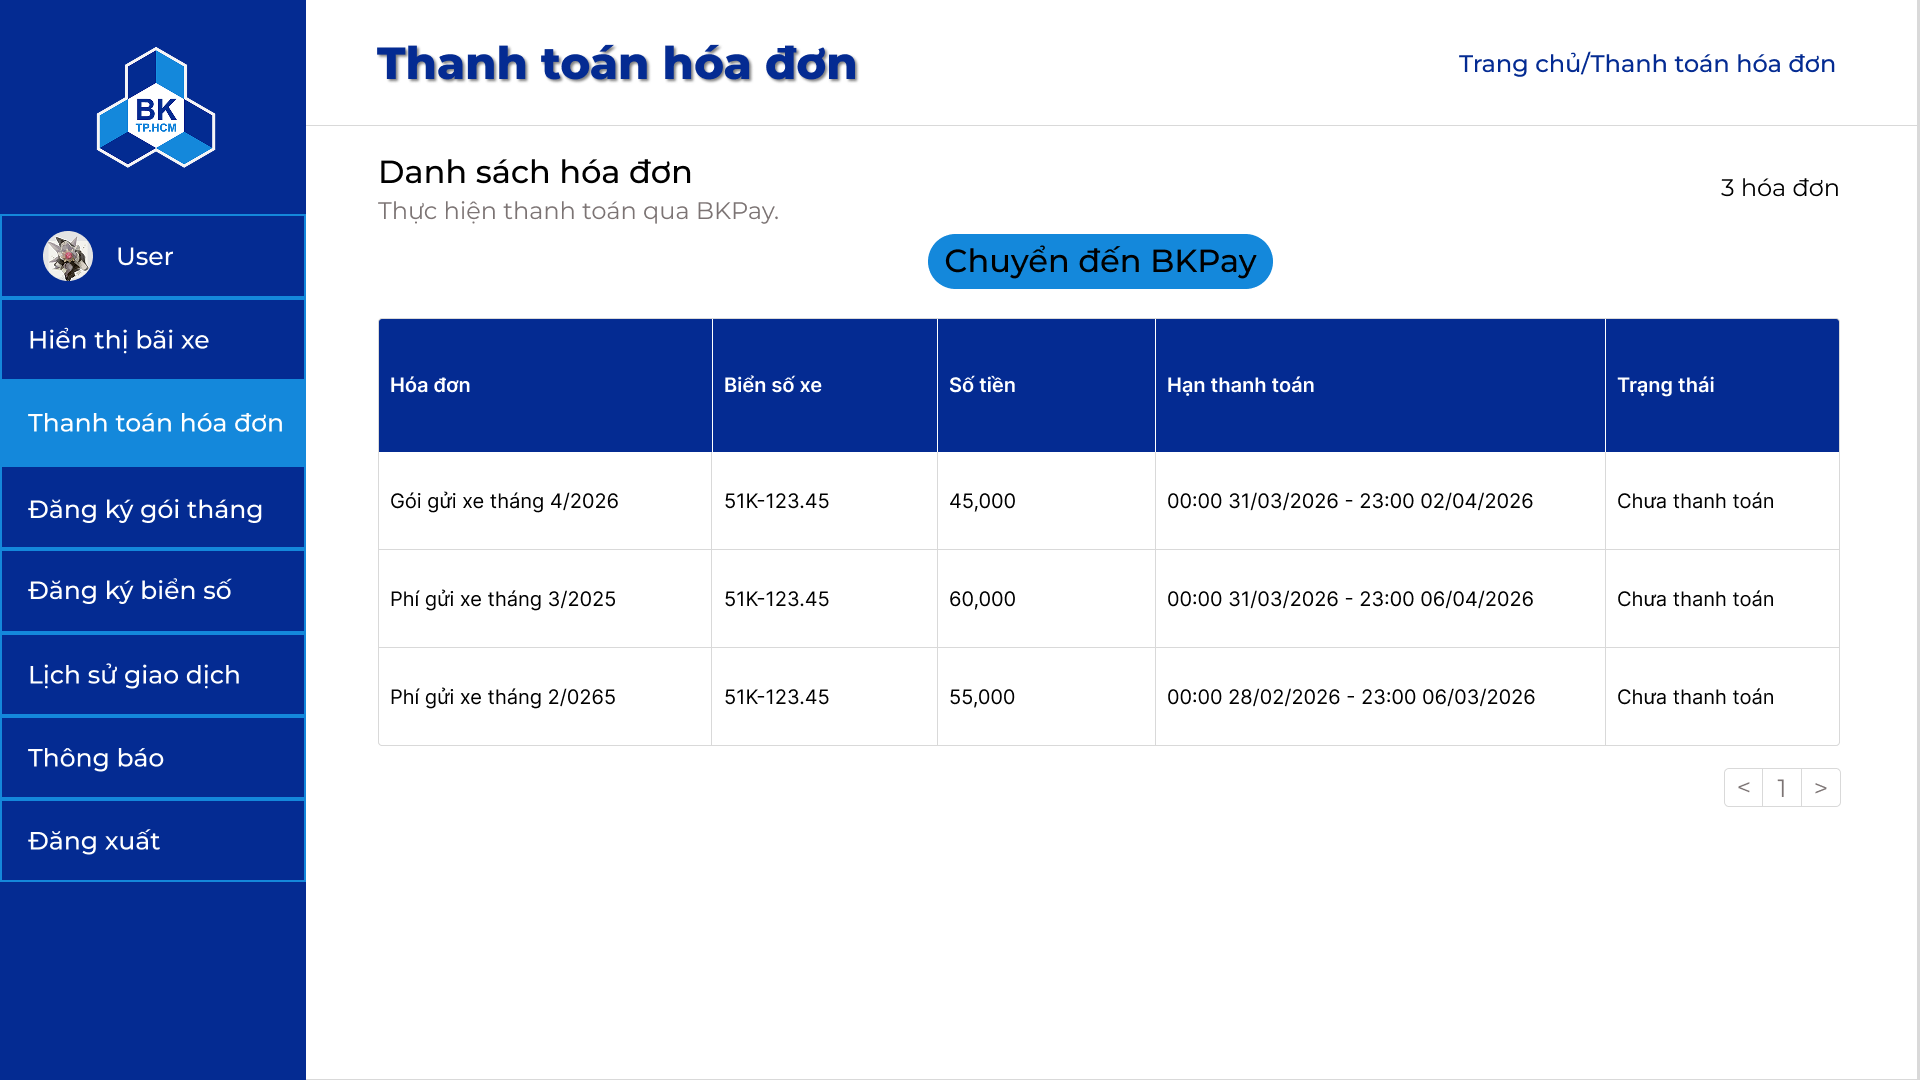
\includegraphics[width=\linewidth]{pictures/thanhtoan.png}
        \caption{Giao diện thực hiện thanh toán hóa đơn}
        \label{fig:login2}
    \end{subfigure}

    \vspace{0.5cm} % Tạo khoảng cách giữa hàng trên và hàng dưới

    % Hàng 2: 2 ảnh tự động căn giữa
    \begin{subfigure}[b]{0.45\textwidth}
        \centering
        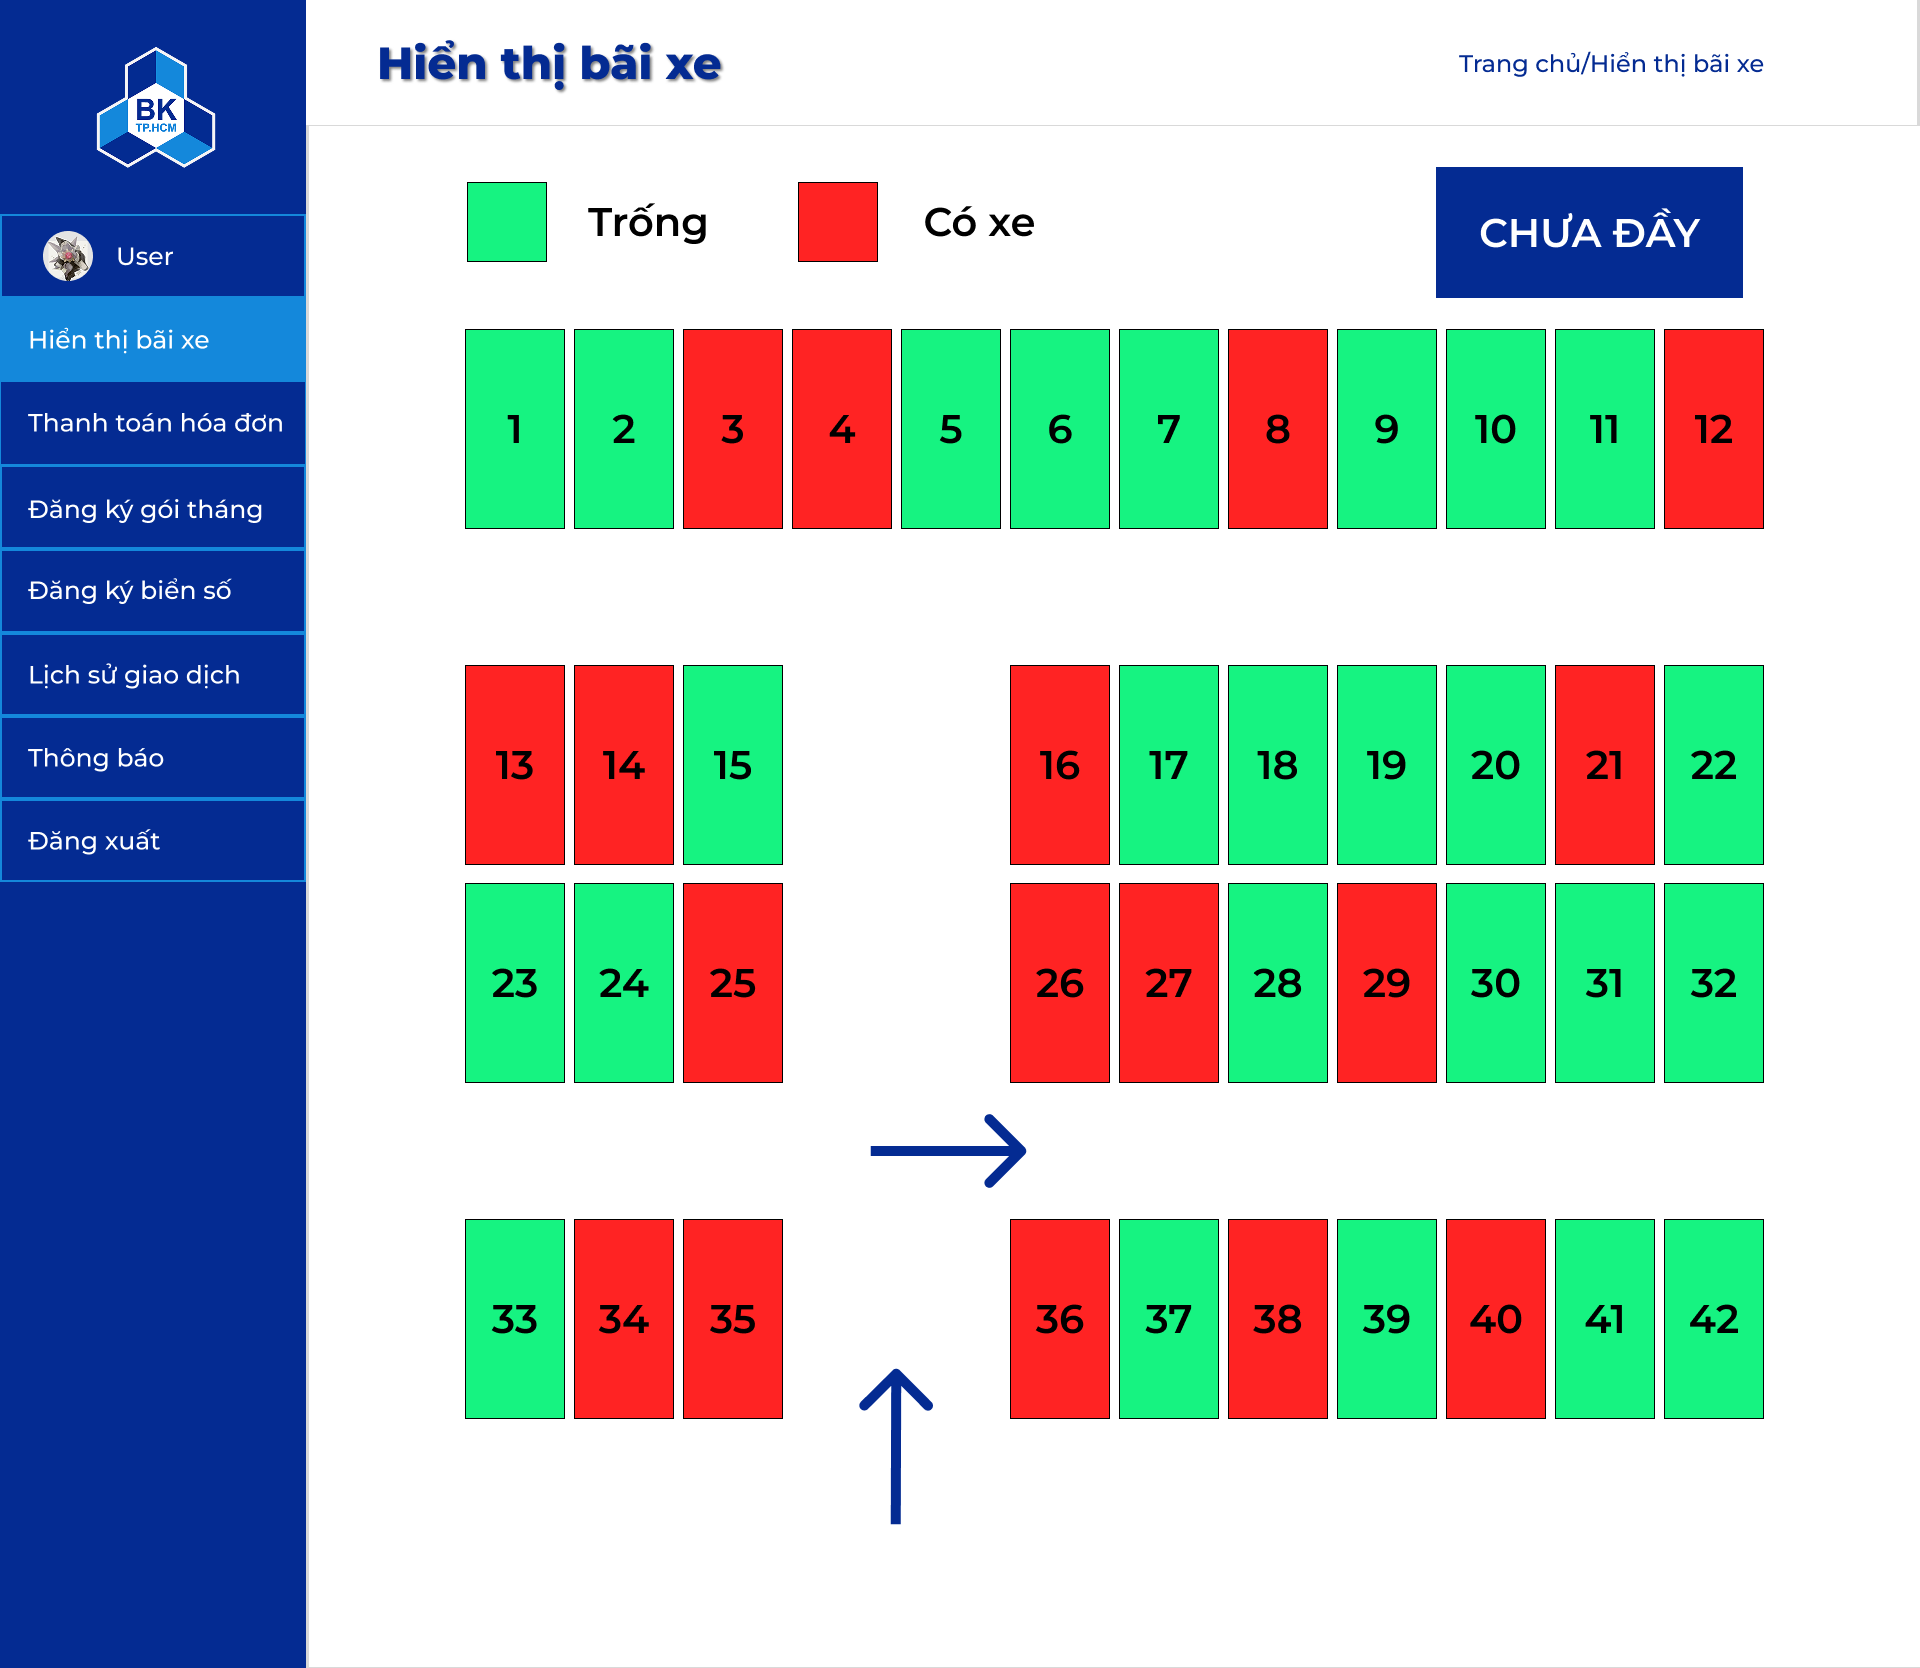
\includegraphics[width=\linewidth]{pictures/baixe.png}
        \caption{Giao diện hiện thị trạng thái bãi xe}
        \label{fig:login3}
    \end{subfigure}
        \hfill
    \begin{subfigure}[b]{0.45\textwidth}
        \centering
        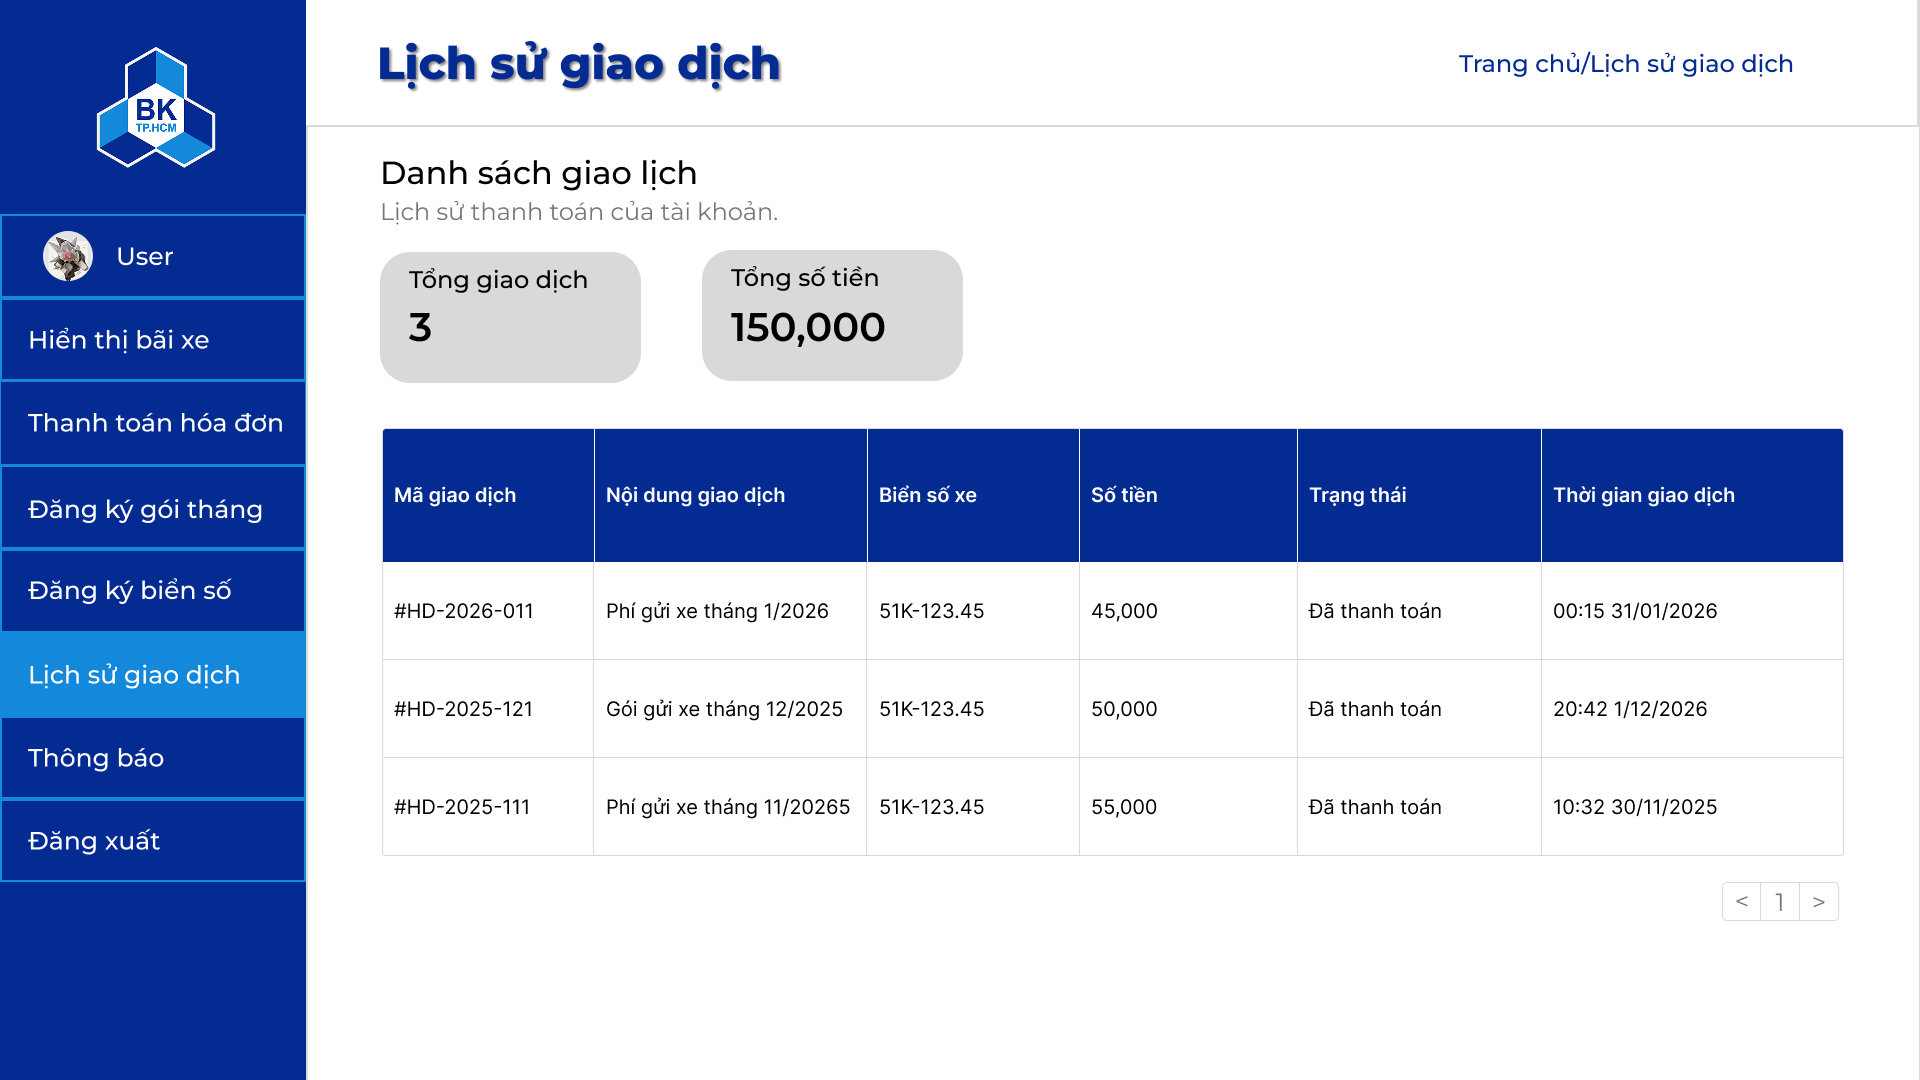
\includegraphics[width=\linewidth]{pictures/History.png}
        \caption{Giao diện lịch sử giao dịch cá nhân}
        \label{fig:login2}
    \end{subfigure}
    
    \caption{Tổng hợp các giao diện cho các tiện ích khác của người dùng}
    \label{fig:three_logins}
\end{figure}

Tại nhóm giao diện này, hệ thống cung cấp các chức năng cốt lõi giúp người dùng chủ động quản lý dịch vụ và các tiện ích bãi đỗ. Cụ thể, người dùng được cấp quyền để thực hiện các thao tác nghiệp vụ sau:
\begin{itemize}
    \item Đăng ký gói dịch vụ
    \item Thanh toán hóa đơn
    \item Tra cứu vị trí đỗ xe
    \item Xem lịch sử giao dịch của bản thân
\end{itemize}



\subsection{Các giao diện cho Admin}


\begin{figure}[H]
    \centering
    % Hàng 1
    \begin{subfigure}[b]{0.3\textwidth}
        \centering
        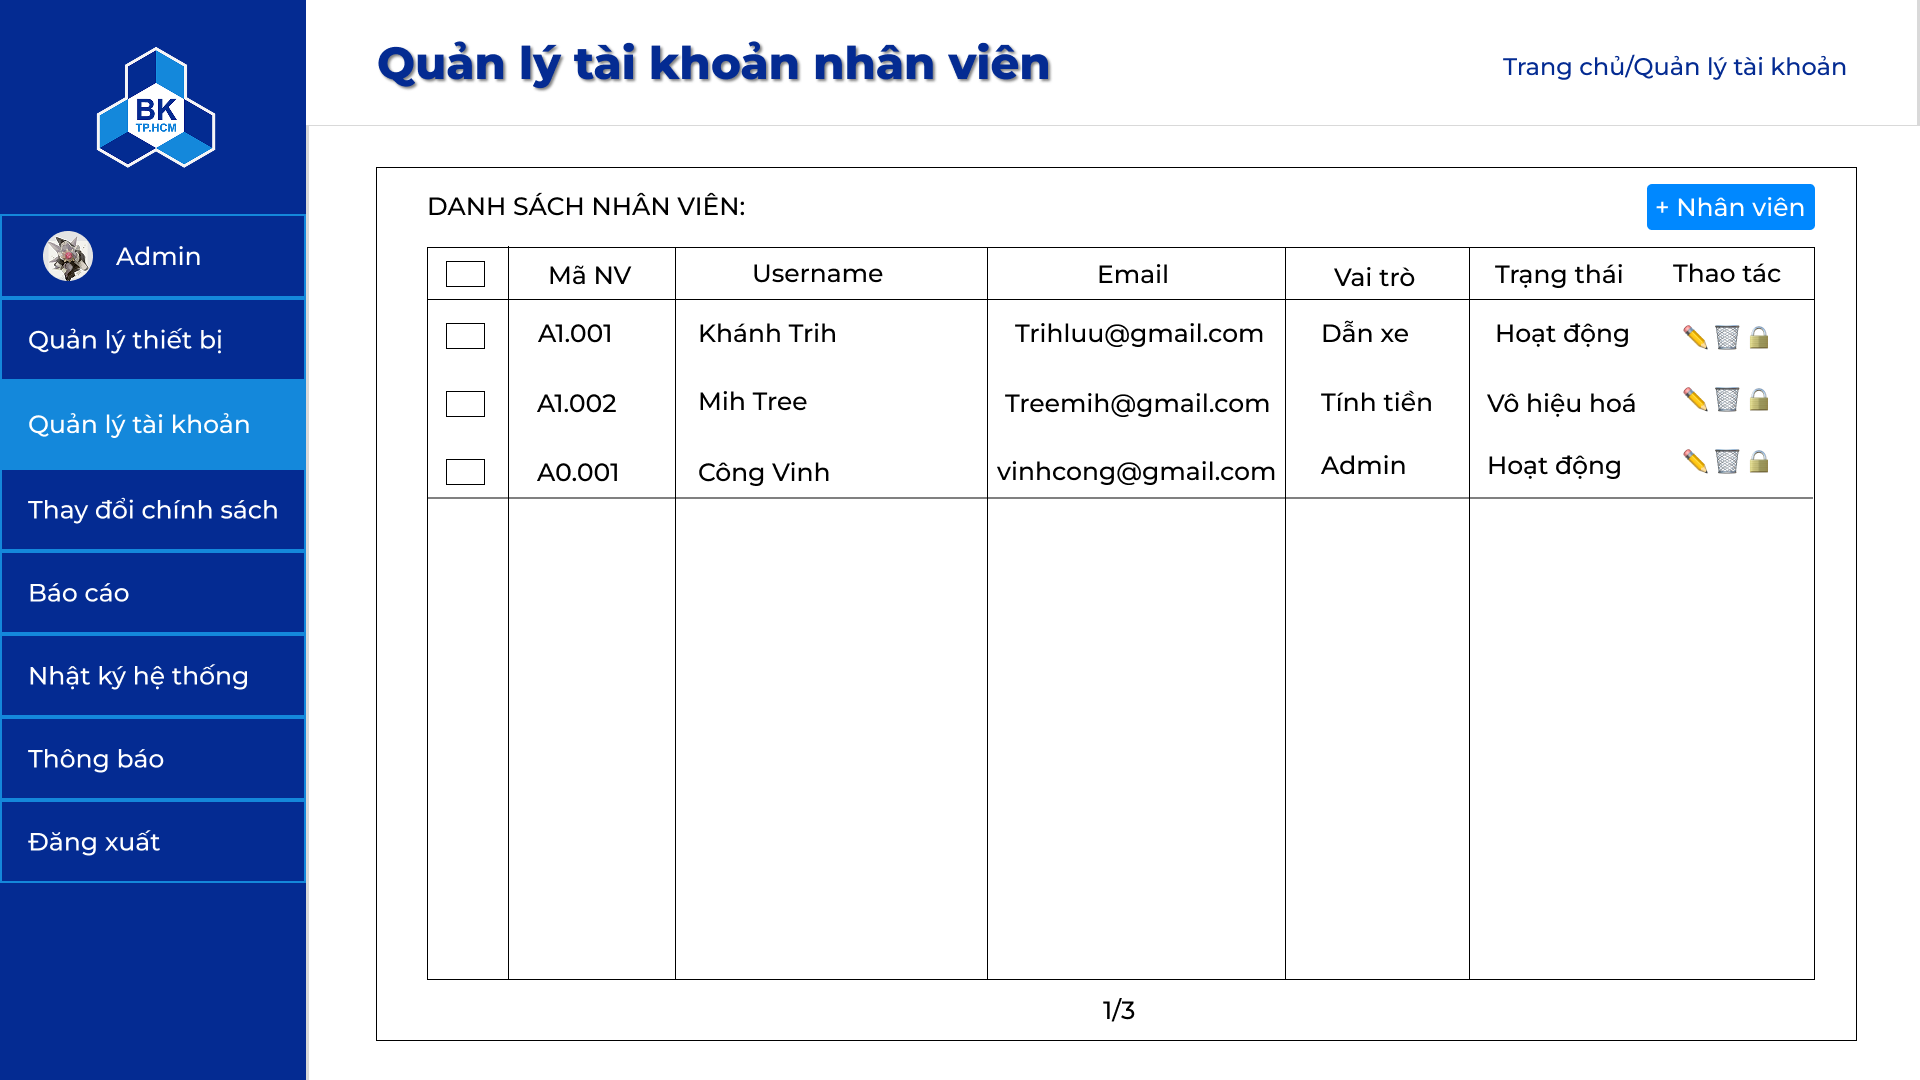
\includegraphics[width=\linewidth]{pictures/QLtknhanvien.png}
        \caption{Giao diện quản lý các tài khoản nhân viên}
    \end{subfigure}
    \hfill
    \begin{subfigure}[b]{0.3\textwidth}
        \centering
        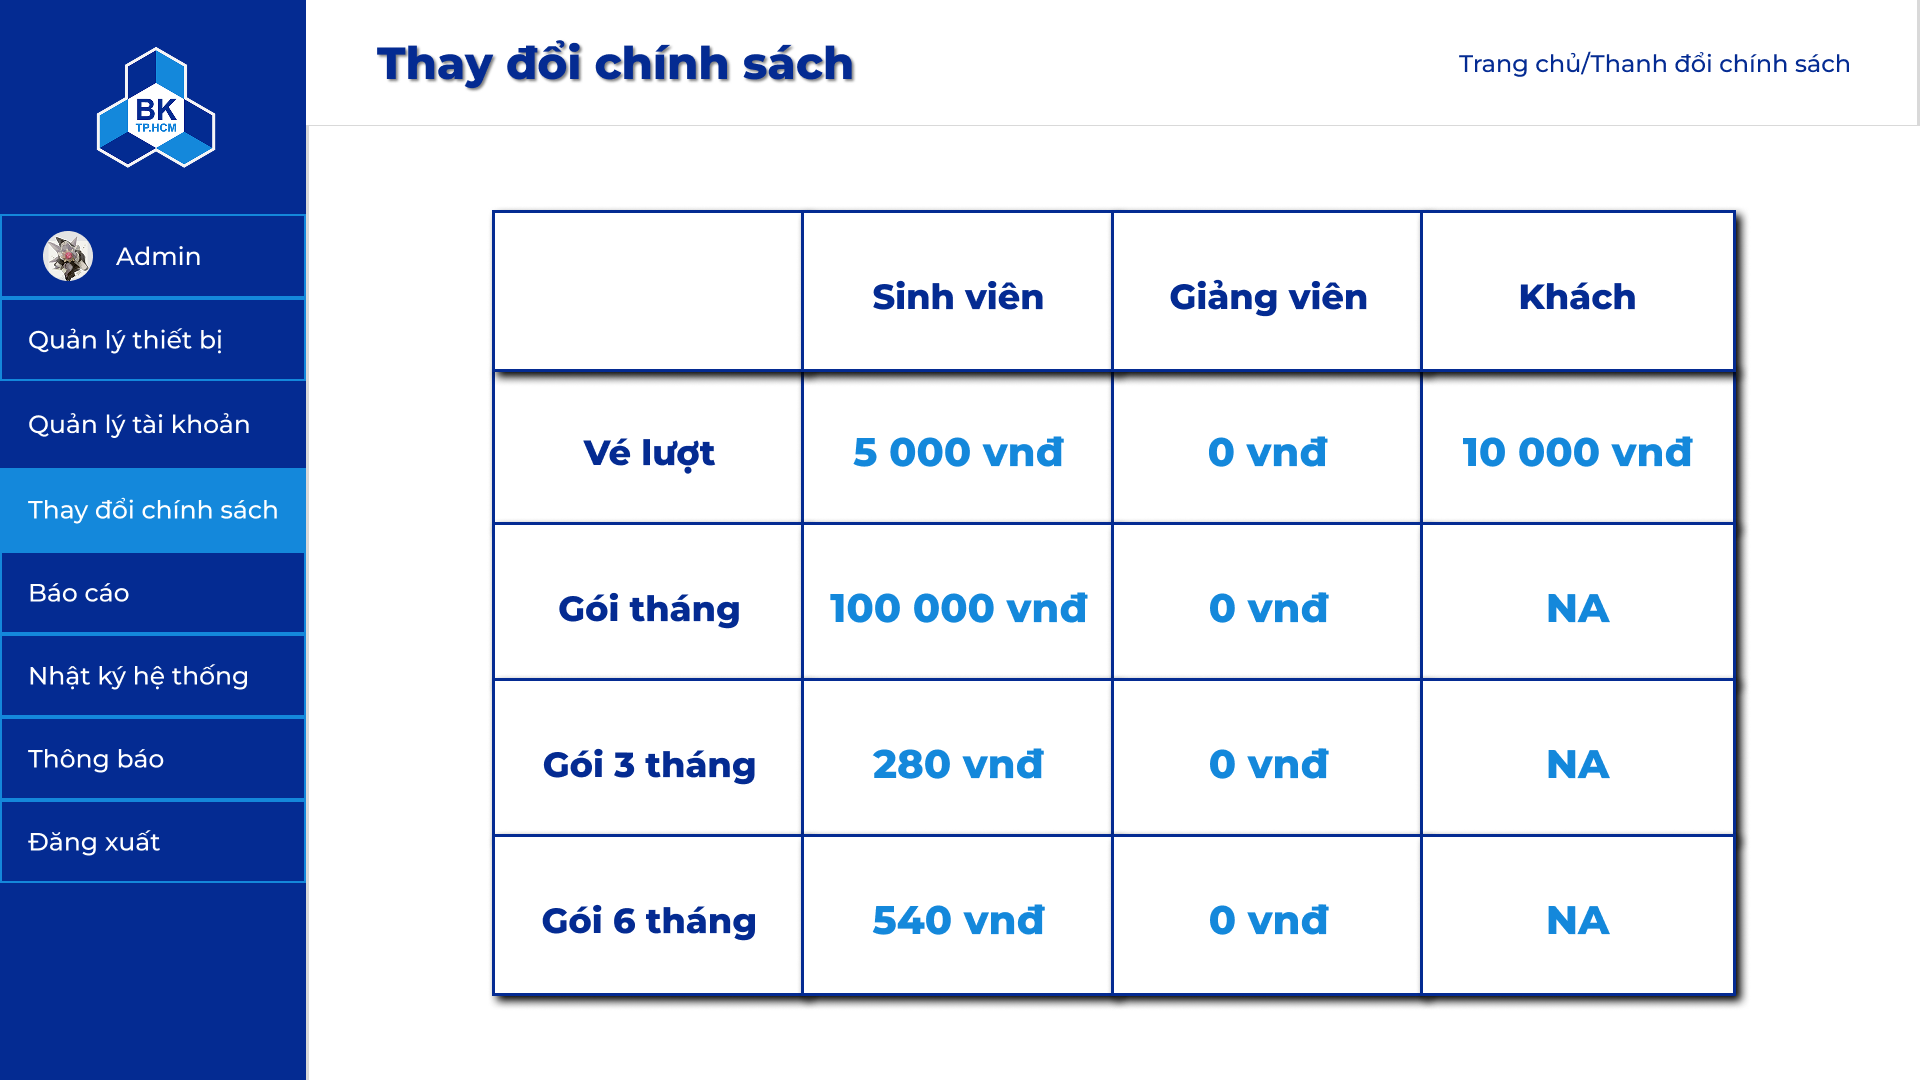
\includegraphics[width=\linewidth]{pictures/Thaydoichinhsach.png}
        \caption{Giao diện nới Admin thay đổi phí gửi xe}
    \end{subfigure}
    \hfill
    \begin{subfigure}[b]{0.3\textwidth}
        \centering
        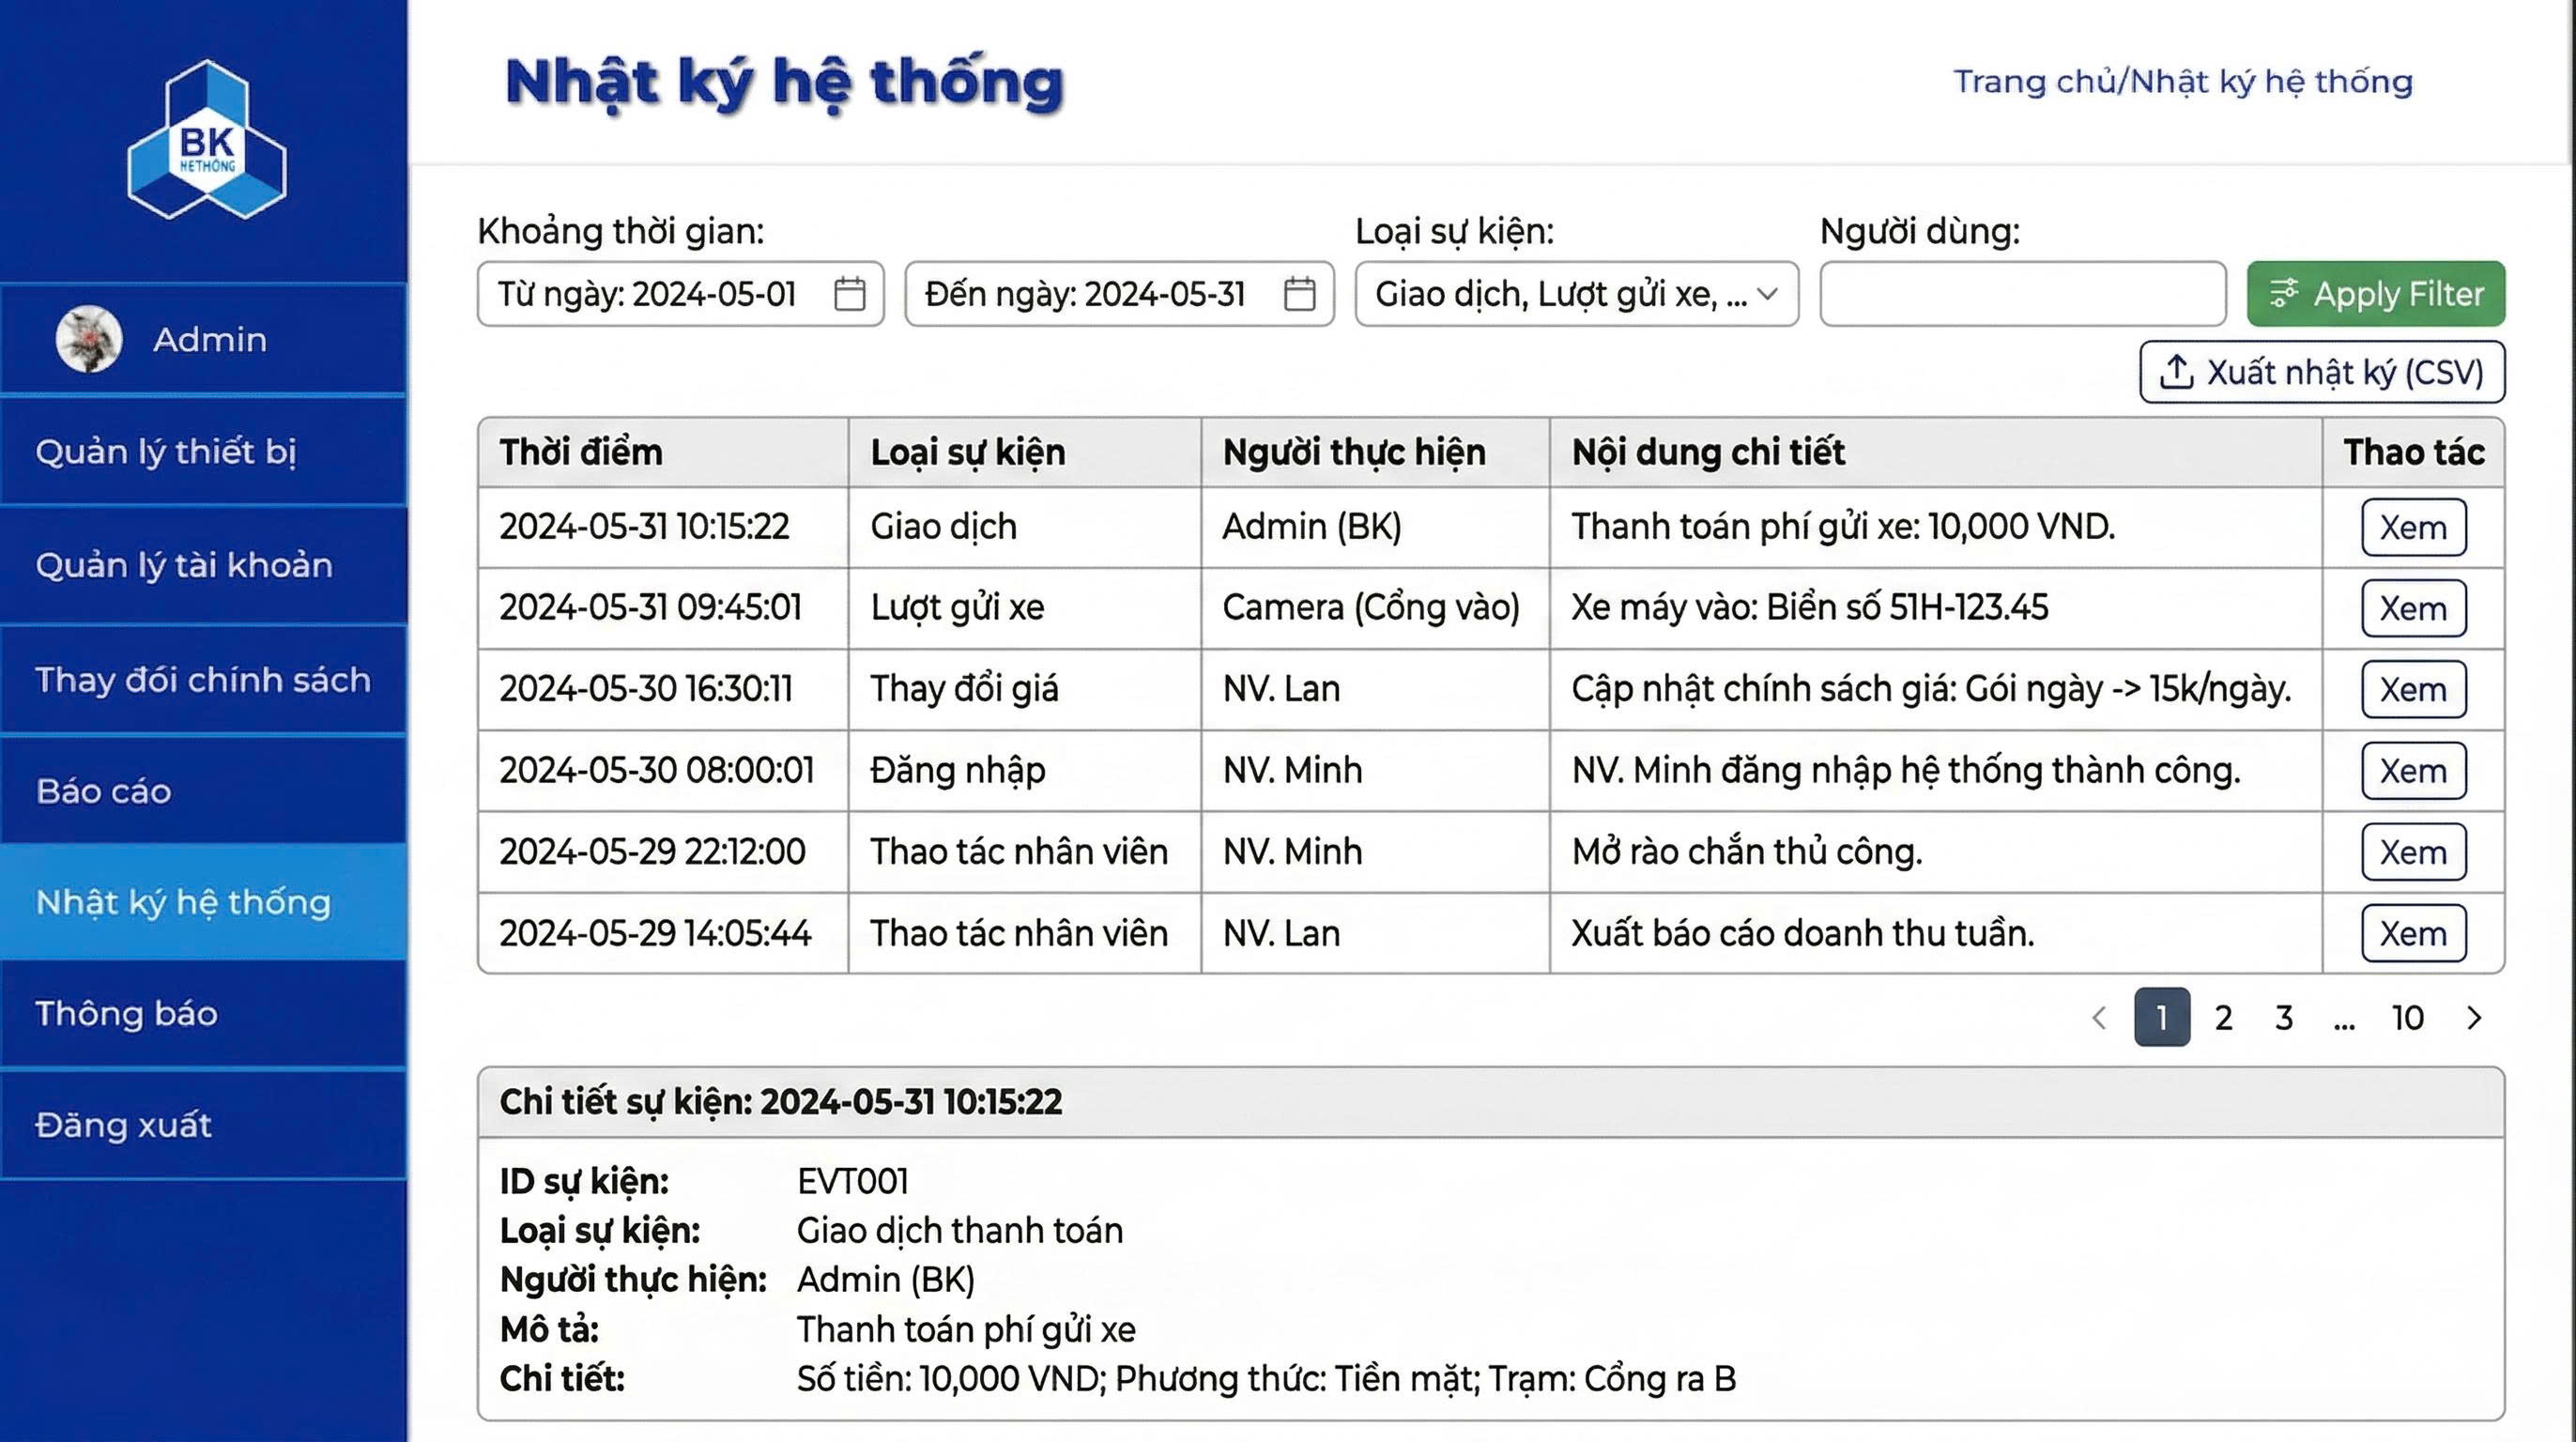
\includegraphics[width=\linewidth]{pictures/nhatky.jpg}
        \caption{Giao diện thông tin nhật ký hệ thống}
    \end{subfigure}

    \vspace{1cm} % Khoảng cách giữa hai hàng

    % Hàng 2
    \begin{subfigure}[b]{0.3\textwidth}
        \centering
        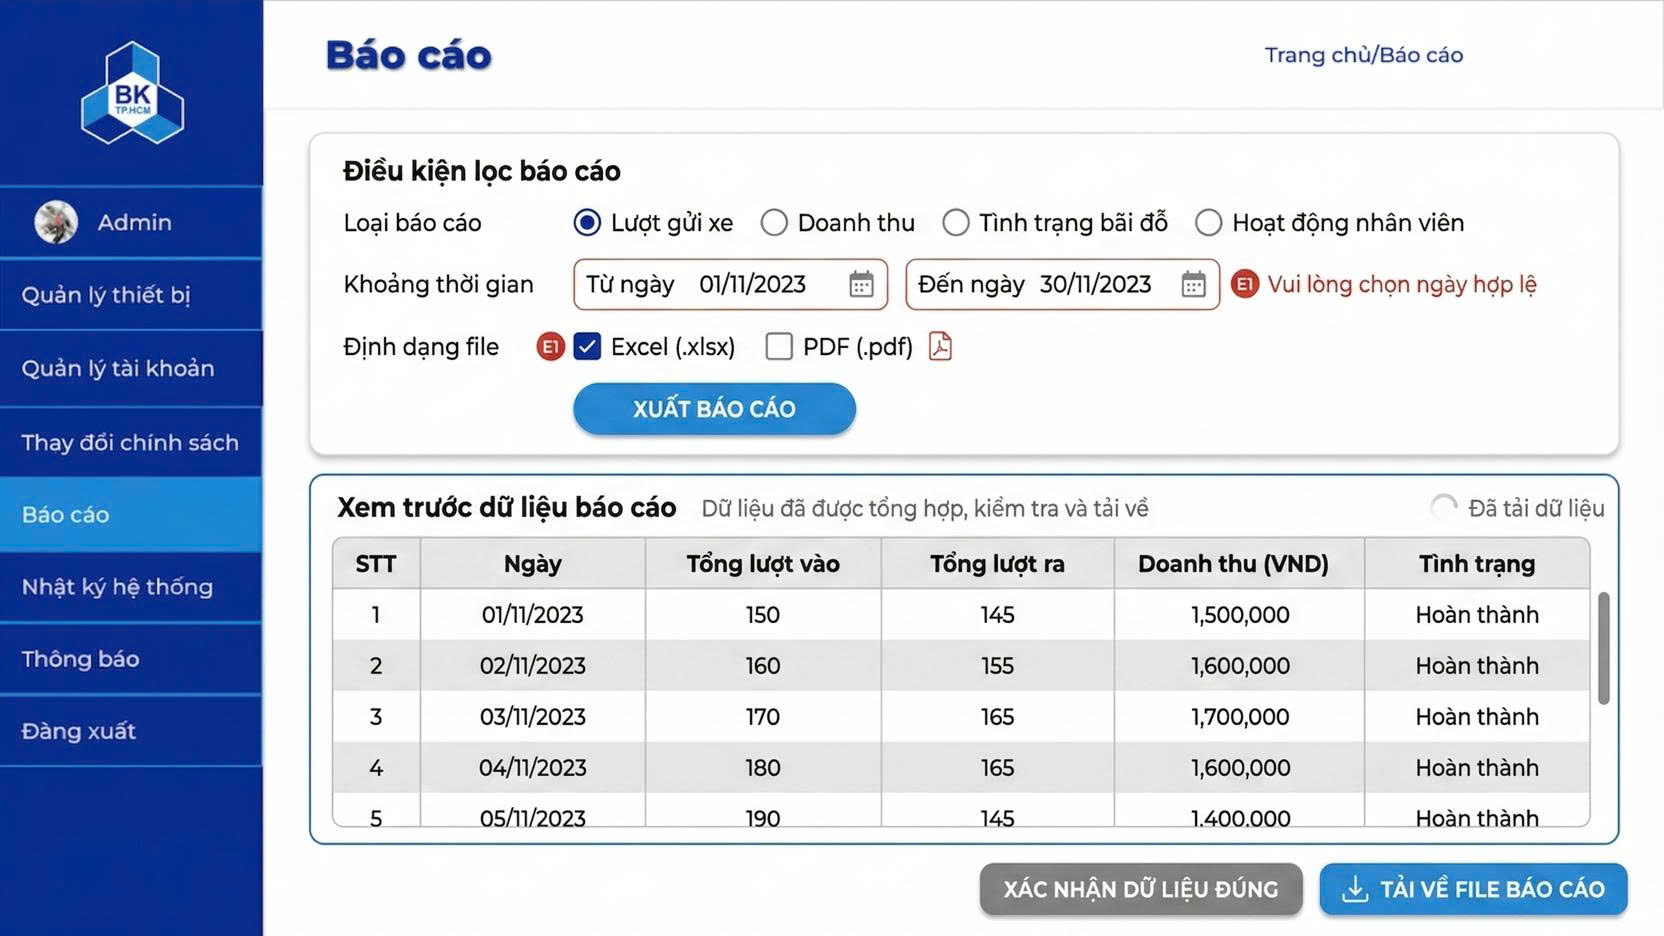
\includegraphics[width=\linewidth]{pictures/baocao.jpg}
        \caption{Giao diện Admin xuất ra các báo cáo cần thiết}
    \end{subfigure}
        \hfill
    \begin{subfigure}[b]{0.3\textwidth}
        \centering
        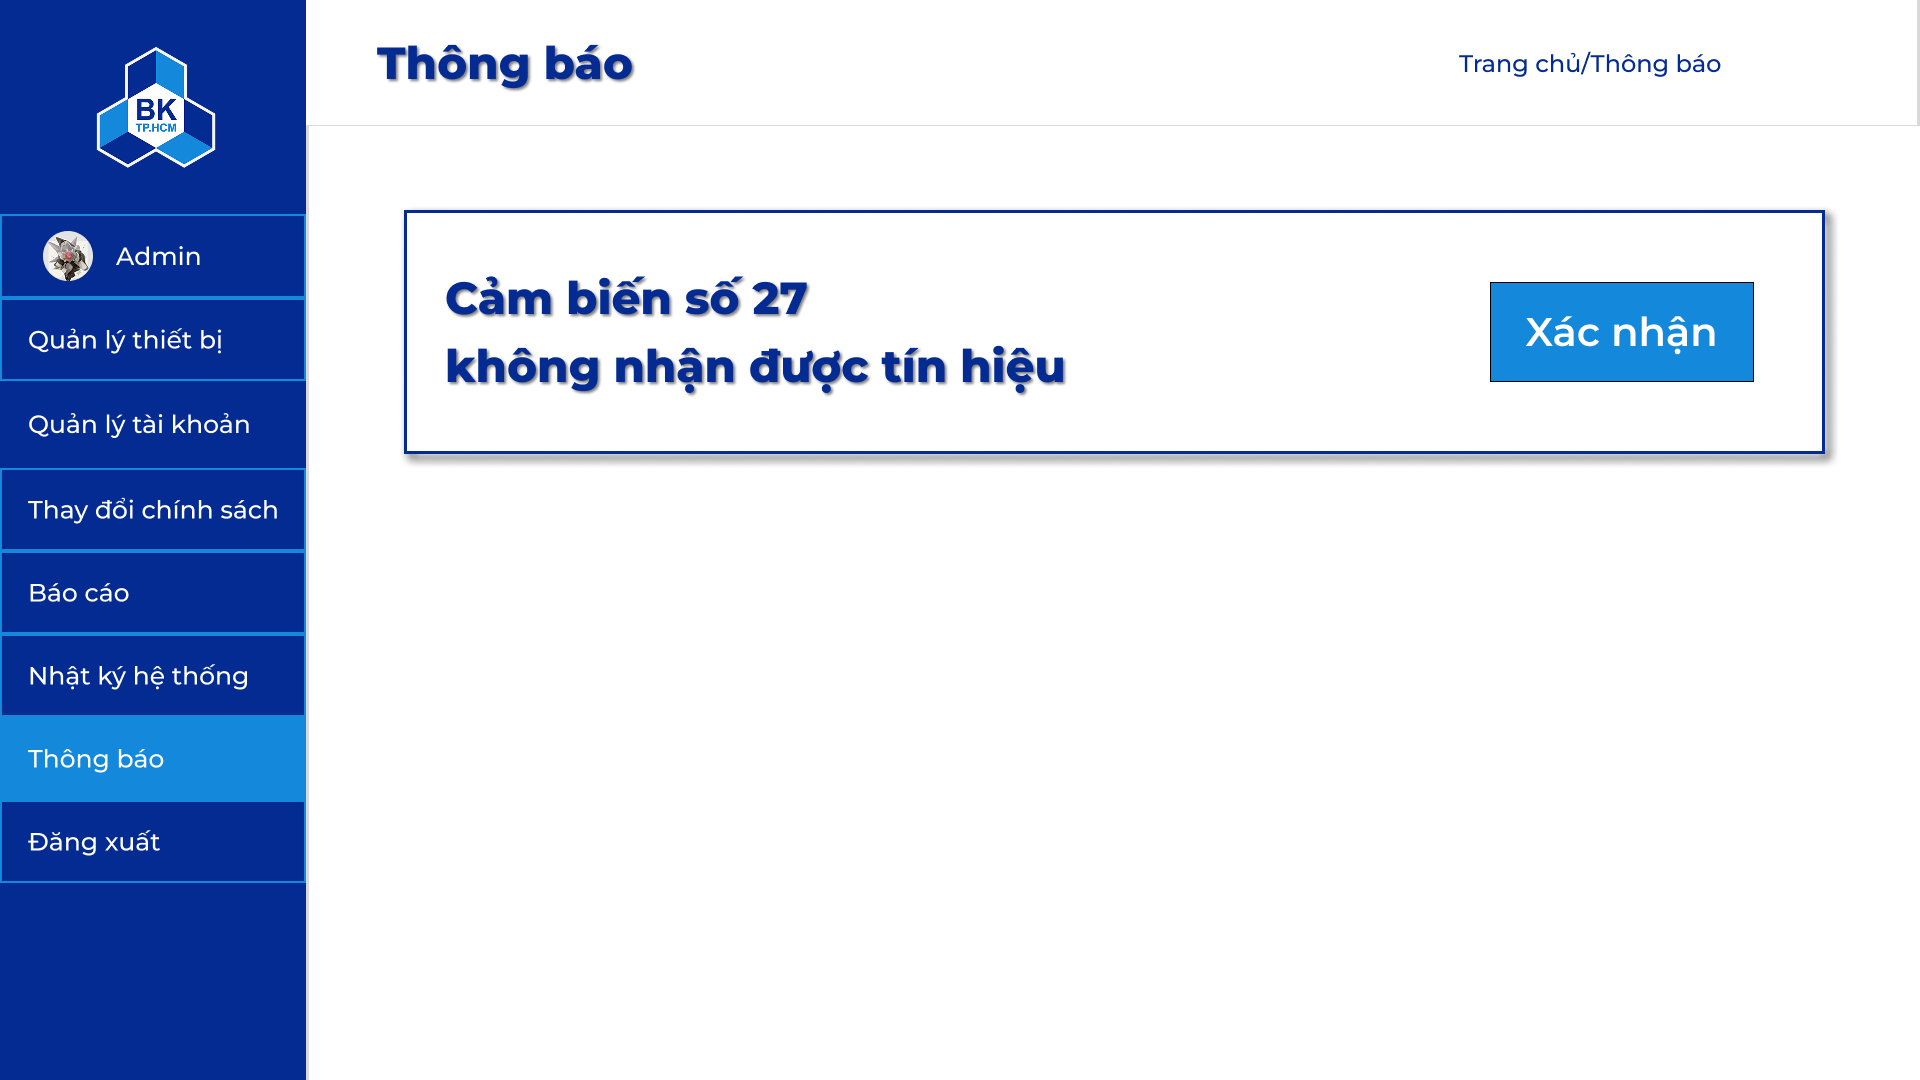
\includegraphics[width=\linewidth]{pictures/notice1.png}
        \caption{Giao diện thông báo khi thiết bị IoT gặp sự cố}
    \end{subfigure}
        \hfill
    \begin{subfigure}[b]{0.3\textwidth}
        \centering
        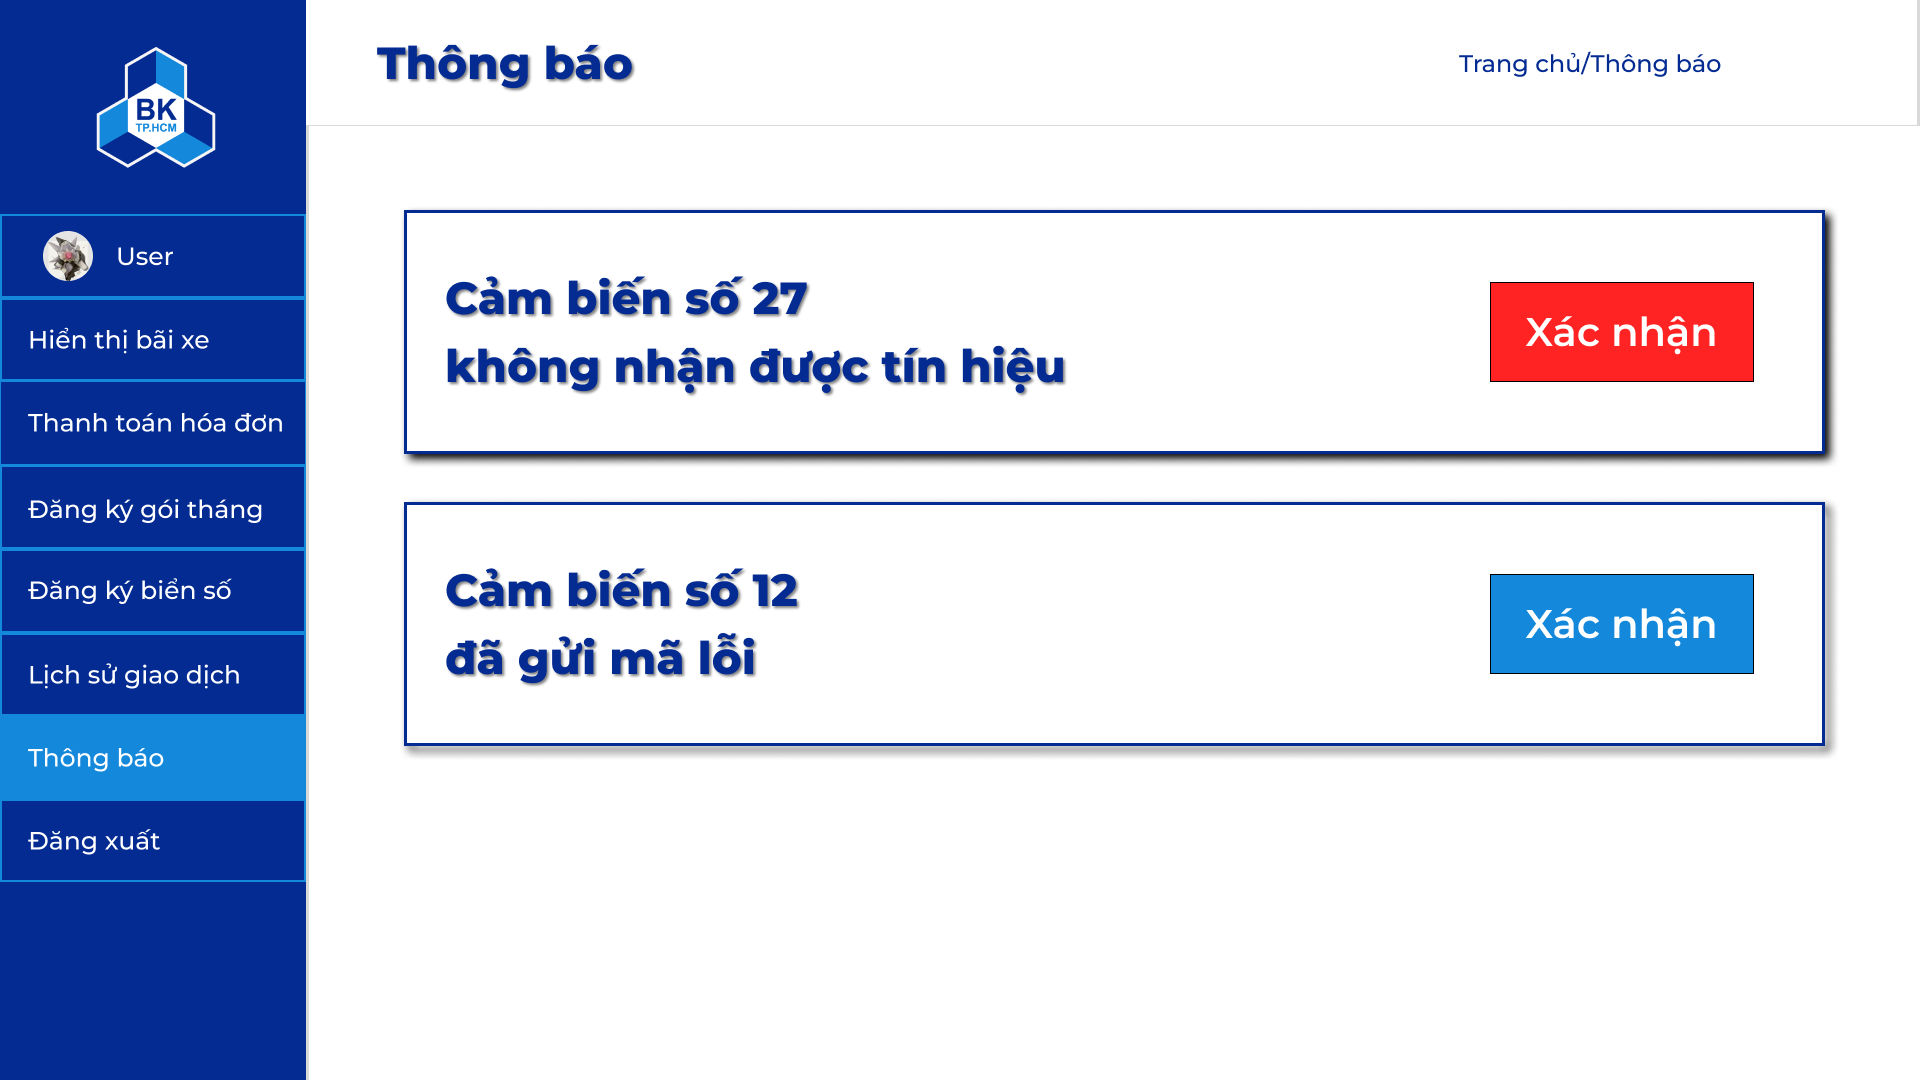
\includegraphics[width=\linewidth]{pictures/notice2.png}
        \caption{Giao diện cảnh báo khi Admin chưa xác nhận các thiết bị IoT lỗi}
    \end{subfigure}

    \caption{Tổng hợp các giao diện cho các chức năng của Admin}
    \label{fig:iot_emergency_workflow}
\end{figure}

Nhóm giao diện dành riêng cho Quản trị viên (Admin) được thiết kế với tiêu chí trực quan, hiện đại và tối ưu hóa trải nghiệm người dùng. Thông qua hệ thống chức năng toàn diện này, Admin có thể dễ dàng thực hiện và kiểm soát mọi hoạt động cốt lõi, từ việc quản lý tài khoản nhân viên, điều chỉnh linh hoạt các chính sách về giá phí, cho đến việc trích xuất báo cáo và theo dõi nhật ký hoạt động chi tiết. Đặc biệt, phân hệ giám sát thiết bị IoT tích hợp cơ chế cảnh báo thời gian thực và nhắc nhở tự động không chỉ giúp Admin nắm bắt ngay lập tức các sự cố phát sinh, mà còn ngăn ngừa rủi ro do sơ suất trong quá trình xử lý, đảm bảo toàn bộ quy trình vận hành luôn diễn ra an toàn, minh bạch và đạt hiệu suất cao nhất.